\section{GP Training Results}\label{sec:results}

With the GP model described in Section \ref{sec:gpmodel},  we train GP models for augmenting the MESA grid (5D GP model). The training data includes the primary and the additional girds as mentioned in Table~\ref{tab:grid}. The role of the additional grid is increasing the grid resolution for evolutionary tracks with the 'hook'. 
%As discussed in the previous section, the kernel function in the 'hook' area are much more complex than other regions , and hence a GP model requires more information to map the feature in this region. 
The total training data includes $\sim$ 15,000 evolutionary tracks and $\sim$ 10,000,000 data points. For validating and testing the data, we computed another 4880 tracks with random model inputs within the grid ranges. These tracks are split 50-to-50 for validating (in the training progress) and testing (after the training progress) GP models.
% We used the same sampling method of training, validating, and testing data. 
In the training process, we use 20,000 training and 20,000 validating data points for each section. 
We do testing when training is completed for sections. The testing dataset contents 50, 000 data points that cover the whole EEP range. Note that we do not use models with $\tau \geq$ 20.0 Gyr, [Fe/H]$_{\rm surf} \leq$ -0.6 dex, or $T_{\rm eff} \geq$ 7000$K$ as testing data. 

\subsection{Overview of Results}

We first train an Exact GP model for the whole grid as a reference. Results of testing errors are listed in Table~\ref{tab:results}. Compared with  2D and 3D GP models, testing errors of this 5D GP model remarkably increase. The results clearly indicate that GP model accuracy declines when input demission increases. 
%
We then train 5D GP models with the section scenario. We gradually increase the number of sections and track changes in testing errors. 
It is found that testing errors are not significantly improved when the data are divided by more than 10 sections as shown in Table~\ref{tab:results}. Comparing testing errors for the 10-, 20-, and 100-sections cases, the 68th and 95th testing errors are at same accuracy levels. Although the 99.7th values slightly decrease for more sections, it is more like a random error.  It turns out that the 10-sections case is the most efficient strategy. Following analysis are all based on this model.   

\begin{table*}
	\centering
	\caption{Training and validating errors for GPR Models}
	\label{tab:results}
	\begin{tabular}{cccccccccc}
		\hline
		Model Type&Inputs&$N_{\rm Training}$ &Sampling rate &\multicolumn{5}{c}{Testing Errors (at 68/95/99.7\%)} \\
		 \hline
		 \multicolumn{4}{c}{}& $T_{\rm eff}$ &$\log g$  &$R$  &[Fe/H]$_{\rm surf}$   &$\tau$ \\
		 \multicolumn{4}{c}{}&  (K)& ($10^{-3}$dex) & ($10^{-3}R_{\odot}$)  &  ($10^{-3}$dex)  & ($10^{-2}$Gyr) \\		 
		 \hline
		 Exact GP & 2D & 20,000 x 1 &96\% & 1/5/11 & 1/3/8 & 2/6/14 & 0.5/2/12 &  1/3/9 \\
		 %SVGP & 2D & 2,000 x 10  &96\% & 1/5/11 & 1/4/10 & 3/7/14  & 0.3/2/14 & 1/4/10  \\
		 \hline		 
		 Exact GP & 3D & 20,000 x 1 & 5\% & 2/6/16 & 1/4/10 & 3/7/17 &  2/6/22 & 2/7/22 \\
		 %Exact GP (5 sections) & 3D & 20,000 x 5 & 20\% & 2/6/17 &1/4/10 & 3/7/16& 1/3/18& 2/6/19\\
		  Exact GP (10 sections) & 3D & 20,000 x 10 & 50\% & 2/5/15 &1/4/11 & 2/7/17& 1/3/20& 2/6/19\\
		% SVGP (too slow) & 3D & 2,000 x 50 & 25\% & 3/7/16 & \\
		 %SVGP (too slow)  & 3D & 5,000 x 20 & 25\% & 2/7/15 & & & & & \\
		 %GIGP (Relu + normal data)& 3D & 100K & 25\% & 2/7/14  & & & & & \\
		 %GIGP (Relu + normal data)& 3D & 200K & 50\% & 4/8/17  & & & & & \\
		 %GIGP (Relu + grid data)& 3D & 220K & 50\% & 5/10/28 & & & & & \\
		 %GIGP (elu + grid data)& 3D & 220K & 50\% & 7/12/29 & & & & & \\
		 %\hline
		 %Exact GP (multitask) & 3D & 20,000 x 1 & 5\% & memory  &  &  &   &  \\
		  \hline		 
		 Exact GP & 5D & 20,000 x 1 & 0.2\% & 3/9/34 & 2/5/18 & 4/11/36 & 2/7/30 & 3/9/27  \\
		 Exact GP (3 sections) & 5D& 20,000 x 3 & 0.6\% &  3/8/27 & 2/5/18 & 3/7/26 & 1/4/24 &3/7/22 \\
		 %Exact GP (3 sections) & 5D& 20,000 x 3 & 0.6\% &  2.5/7.7/27.4 & 15/45/177 & 26/73/257 & 9/42/236 &26/73/226 \\
		 Exact GP (5 sections) & 5D& 20,000 x 5 & 1\% &  2/7/25 & 1/4/15 & 3/7/24 & 1/4/21 &2/6/22 \\
		 %Exact GP (5 sections) & 5D& 20,000 x 5 & 1\% &  2.4/7.2/24.8 & 13/39/152 & 25/71/242 & 9/39/207 &21/64/215 \\
		 Exact GP (10 sections) & 5D& 20,000 x 10 & 2\% & 2/7/27  & 1/4/14 & 2/7/26 &1/4/20 & 2/6/21\\
		 %Exact GP (10 sections) & 5D& 20,000 x 10 & 2\% & 2.4/7.1/26.8  & 14/40/141 & 24/70/263 &9/37/196 & 21/64/208\\
		 Exact GP (20 sections) & 5D& 20,000 x 20 & 4\% & 2/7/26  & 1/4/14 & 2/7/27 &1/3/18 & 2/6/22 \\
		 %Exact GP (20 sections) & 5D& 20,000 x 20 & 4\% & 2.2/6.9/26.1  & 13/38/141 & 24/72/290 &9/32/182 & 19/61/218 \\
		  Exact GP (100 sections) & 5D& 20,000 x 100 & 20\% & 2/7/25  & 1/4/14 & 2/7/26 &1/3/17 & 2/6/18 \\
		 % Exact GP (100 sections) & 5D& 20,000 x 100 & 20\% & 2.2/6.7/25.8  & 13/36/157 & 23/67/283 &8/34/185 & 19/59/190\\
		 %GIGP (Elu) & 5D & 10 x10,000 & 1\% & 5/12/34 & & & & \\
		 %GIGP (Relu) & 5D & 10 x10,000 & 1\% & 6/13/47 & & & & \\
		 %GIGP & 5D &  & 2\%, 5\%, 10\%, 25\%  & memory & & & & \\
		% \hline
		 % \multicolumn{9}{c}{GP a subset of 5D data-hook}\\
		 %\hline
		 %Exact GP EEP = 0.2-0.4 & 5D & 20,000 x 1 & 1\% & 2/7/20 &&&\\
		 %Exact GP EEP = 0.3-0.4 & 5D & 20,000 x 1 & 2\% & 3/8/21  &&&\\
		 %Exact GP EEP = 0.3-0.35 & 5D & 20,000 x 1 & 3\% & 2/7/17 &&&\\
		  %Exact GP EEP = 0.3-0.32 & 5D & 20,000 x 1 & 8\% & 2/5/14 &&&\\
		 %Exact GP EEP = 0.3-0.31 & 5D & 20,000 x 1 & 16\% & 2/4/13  &&&\\
		  \hline
	\end{tabular}
\end{table*}

\begin{figure*}
	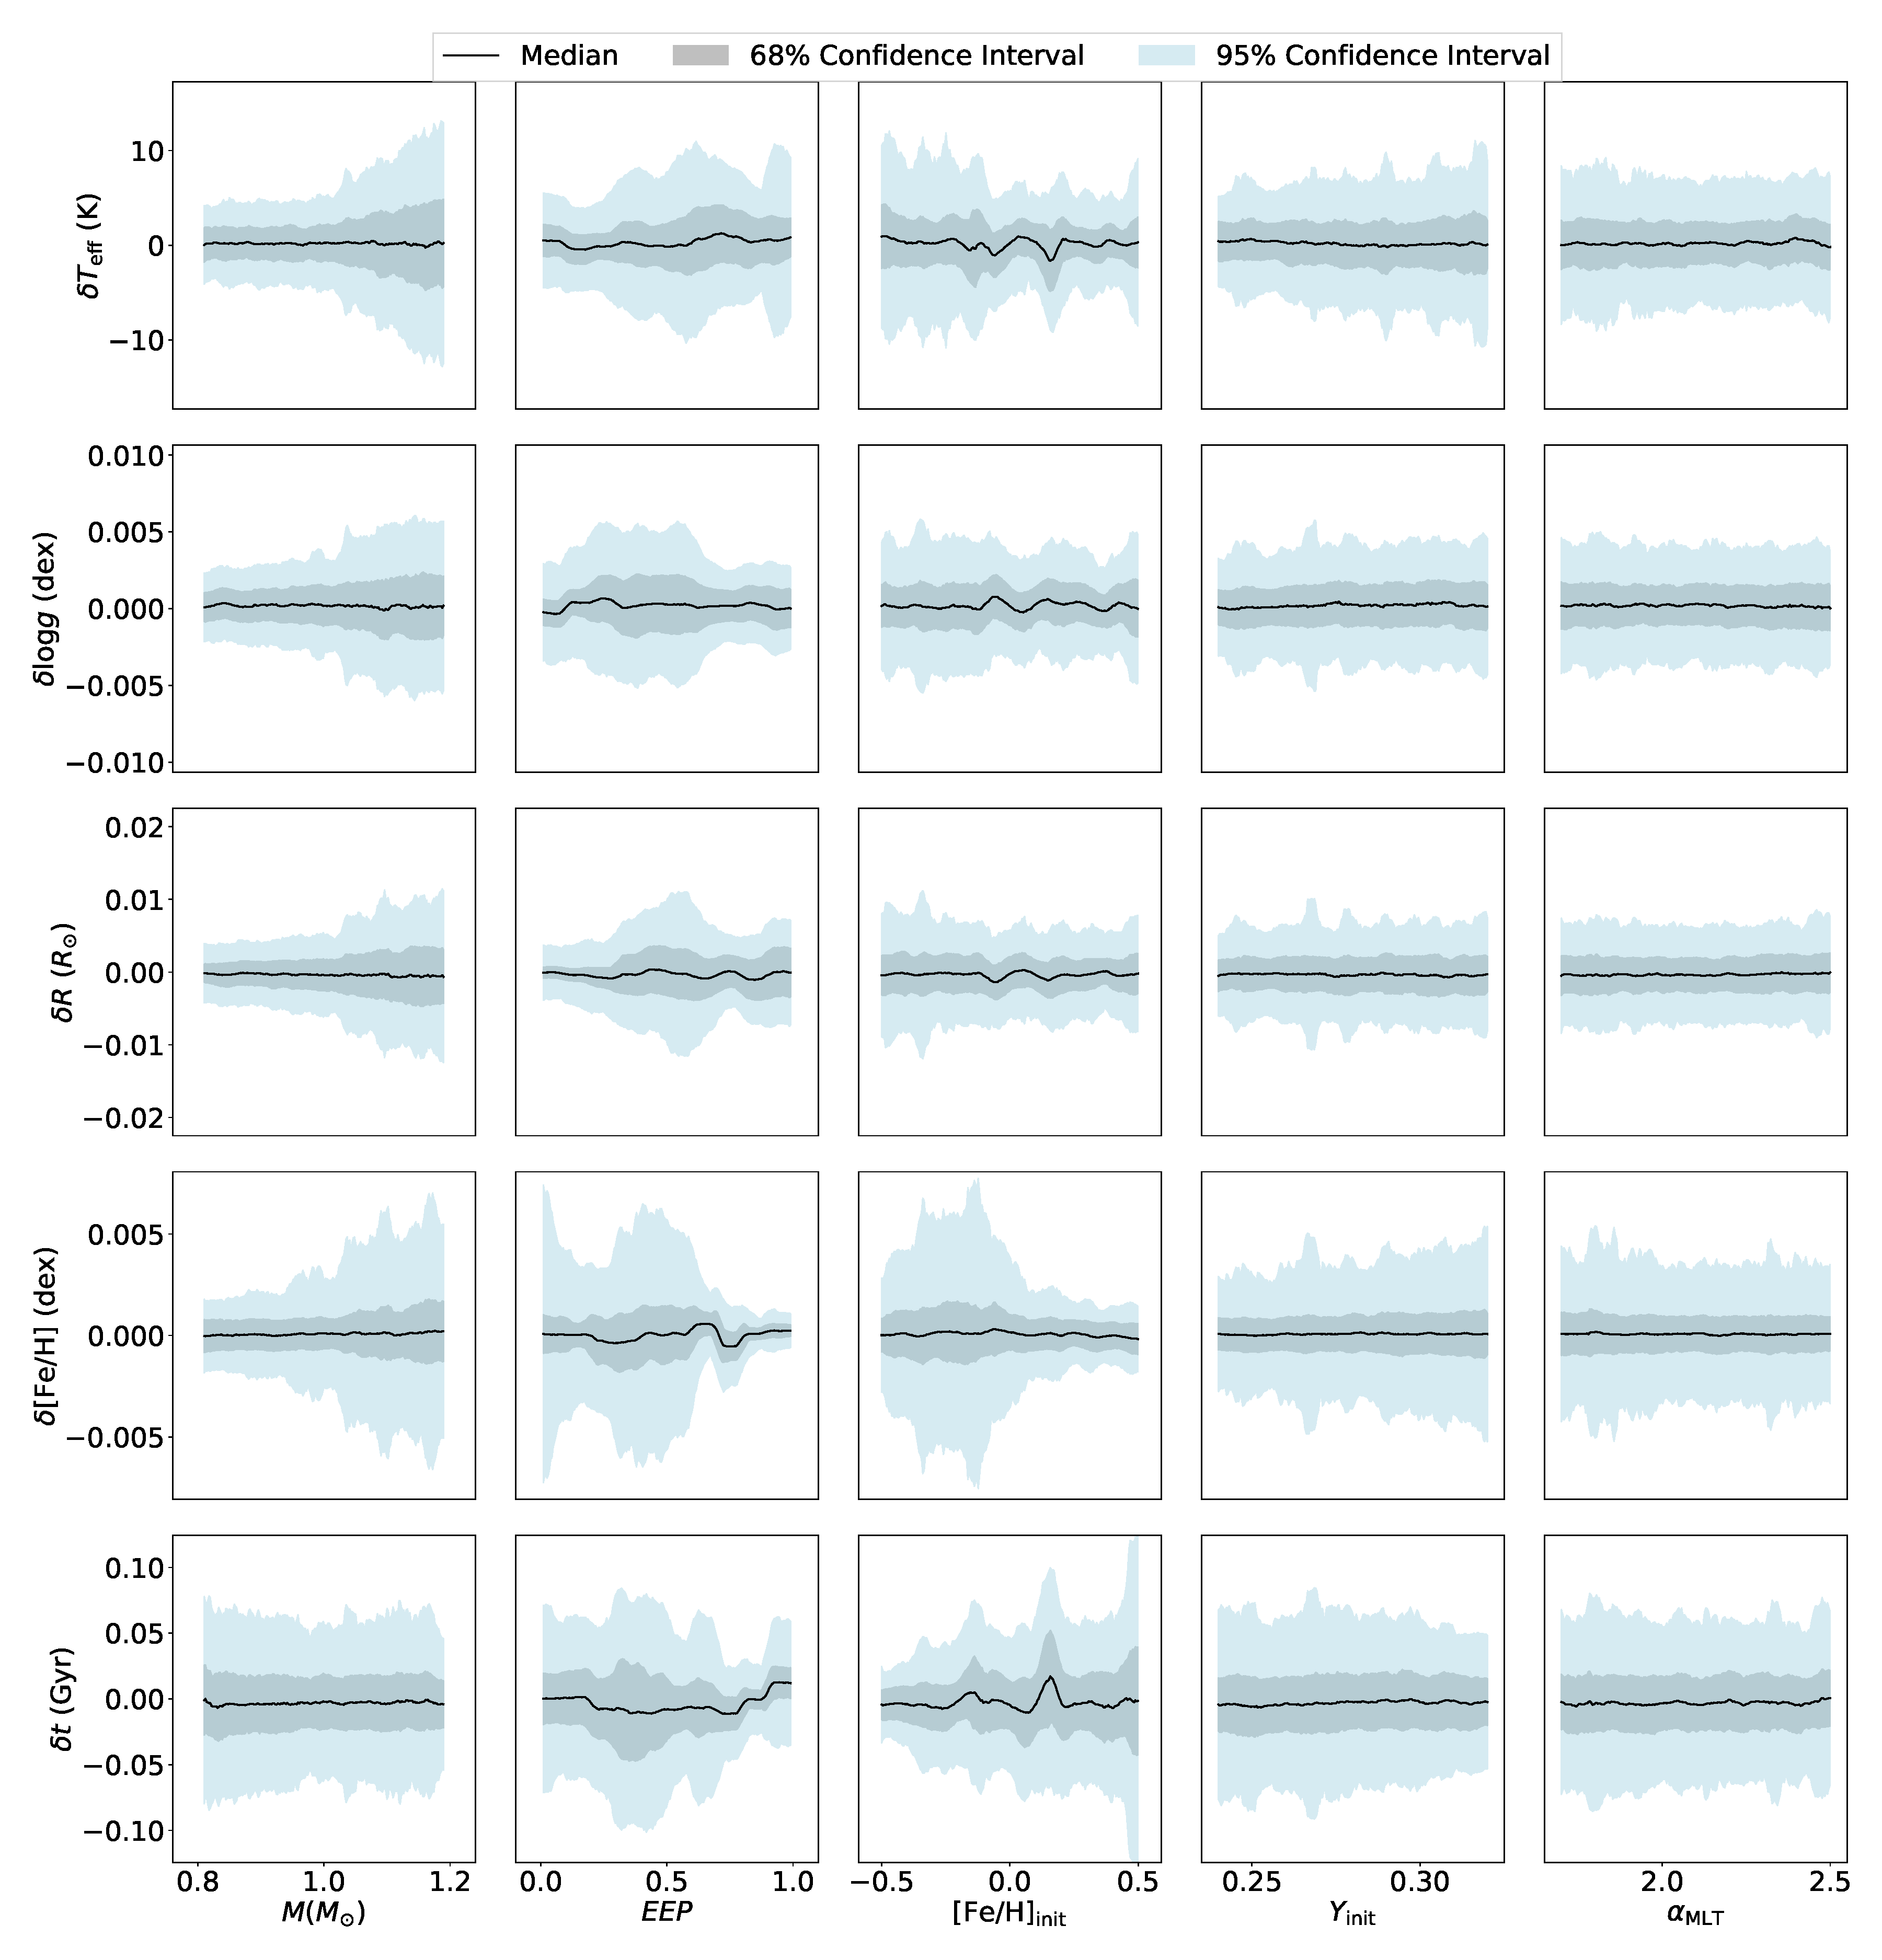
\includegraphics[width=2.0\columnwidth]{ 5d-testing_vs_inputs.pdf}
    \caption{ Roll medians and confidential interval of testing errors against GP model  inputs. Black solid line indicate the median; grey and blue shadow represent the 68\% and 95\% confidential interval. Testing errors of $T_{\rm eff}$, $\log g$, and $R$ mainly depend on $M$ and $EEP$. Metallicity error strongly depends on $M$, $EEP$, and [Fe/H]$_{\rm init}$, and age error has a significant correlation to $EEP$ and [Fe/H]$_{\rm init}$. However, testing errors do not obviously relate to $Y_{\rm init}$ or $\alpha_{\rm MLT}$. } 
  \label{fig:5d_test_vs_input}
\end{figure*}


A overview of the GP model accuracy can be seen in Figure~\ref{fig:5d_test_vs_input}, in which we demonstrate rolling medians and standard deviations of testing errors of each output as a function of each input parameter.
%
It can be seen that the median values are approximate along zero in most plots, indicating that there is no obvious systematic offsets.
%
The 68\% confidential intervals are generally small and do not significantly vary. However, the 95\% confidential intervals change in a in larger dynamic ranges and clearly depends on $M$, $EEP$, and $\rm [Fe/H]_{init}$. This is caused by the tail feature as illustrated in Figure~\ref{fig:2dtest}. It turns out that the marginal error distributions is not a good way to estimate systematic uncertainties for GP outputs. 
%

\subsection{Mapping Systematical Uncertainties across the input parameter space}\label{sec:sys}

Systematical uncertainties of GP model are not uniform as shown in Figure~\ref{fig:5d_test_vs_input}. They relate to $M$, $EEP$, and [Fe/H]$_{\rm init}$ but not to $Y_{\rm init}$ or $\alpha_{\rm MLT}$.  Thus, a comprehensive statistical model for systematical uncertainty can be described as a function of $M$, $EEP$, and [Fe/H]$_{\rm init}$. 
%

We examine local error distributions in the $M$-$EEP$-$\rm [Fe/H]_{init}$ space. We divided this space into equal-size segments. The the choice of the segment size matters. It needs to be small enough for only presenting the local feature, but it can not be very small so that there are not enough data points for proper statistical analysis. 
%
To find the appropriate size, we do a statistic test for the data in every segment to test wether the local error distribution has a tail feature. The condition we apply for the test is either the ratio between 68\% confidential interval and 95\% confidential interval less than 2.5, or the ratio between 68\%  confidential interval and 99.7\% confidential interval less than 4. 
%
After several attempts, we decide to divide the input range into 40 equally spaced segments for $M$, 50 for $EEP$, and 20 for [Fe/H]$_{\rm init}$. Hence there are 43,911 (41 x 21 x 51) points in the space. Local standard deviation for each point is computed with the data in a 3-segments (1.5 previous and 1.5 after) range.  The statistic test shows that $\sim 90\%$ points meet the above condition. This infer that the selection of segment size statistically sounds.  

%
We demonstrate local systematic uncertainties of testing errors for $T_{\rm eff}$ ($\sigma T_{\rm eff}$) on the $M-EEP$ diagram in Figure \ref{fig:5d_sys_teff}. As it can be seen that $\sigma T_{\rm eff}$ values are below $\sim 4 K$ in the low-mass regions and raise when mass is greater than 1.05$M_{\odot}$. The distribution is smooth in general but there are many substructures on the diagram. We also do visual inspections for the error distributions of other outputs and all of the show various substructures across the 3D space. It is apparently not convinced to describe the error distribution with any simple mathematical expressions. We hence use another GP model (GP-SYS model) to map three fundamental inputs ($M$, $EEP$, and [Fe/H]$_{\rm init}$) to local systematic uncertainty of each output.   

Here we discuss how we set up the GP-SYS model. 
%
There are 43,911 data points and we split them for training and validating. We randomly select 32,000 data points as the training dataset and use the rest 11,311 data points as the validating dataset. Because the training data size exceeds the 20,000 limit for Exact GP, we need other approach for the large data sample.
%
As mentioned in Section \ref{sec:gpmodel}, the SVGP framework works when the dataset is large and the kernel function is not very complex. It hence suitable for this case. We use 10,000 inducing points which are randomly selected in the 3D space. The training data is divided into 10 random batches for the SVGP training. In each training iteration, the 10 data batches is feeded in by turn to optimises hyperparameters. 
%
We use a constant mean function and the RBF kernel for this GP-SYS model because we want a smooth function to describe the systematic uncertainty. The variational evidence lower bound (ELBO) is adopted as the loss function. This approach is designed for when there is too much data for exact inference. The Early Stopping which is controlled by RMSE value of validating data. The training progress terminates when the validating RMSE stops decreasing for 30 iterations.
We set up the likelihood function and the optimiser with the same method as training the GP-Grid model. 
Our set up for the GP-SYS model is listed as follow.
\begin{itemize}
\item Model Type: SVGP with 10,000 inducing number. 
\item Model Inputs: $M$, $EEP$, and [Fe/H]$_{\rm init}$
\item Model Outputs: $\sigma_{T_{\rm}}$, $\sigma_{\log g}$, $\sigma_{R}$, $\sigma_{\rm [Fe/H]_{surf}}$, and $\sigma_{\tau}$.
\item Training dataset: 3200 x 10 data points
\item Validating dataset: 11,311 data points
\item Kernel: RBF (for all outputs)
\item Mean Function: Constant Mean Function 
\item Likelihood Function: Gaussian Likelihood Function
\item Loss Function: The variational evidence lower bound (ELBO) 
\item Optimiser: Adam including AMSGRAD variant
\item Early Stoping: when validating RMSE stops decreasing for 30 iterations
\end{itemize}    


\begin{figure}
	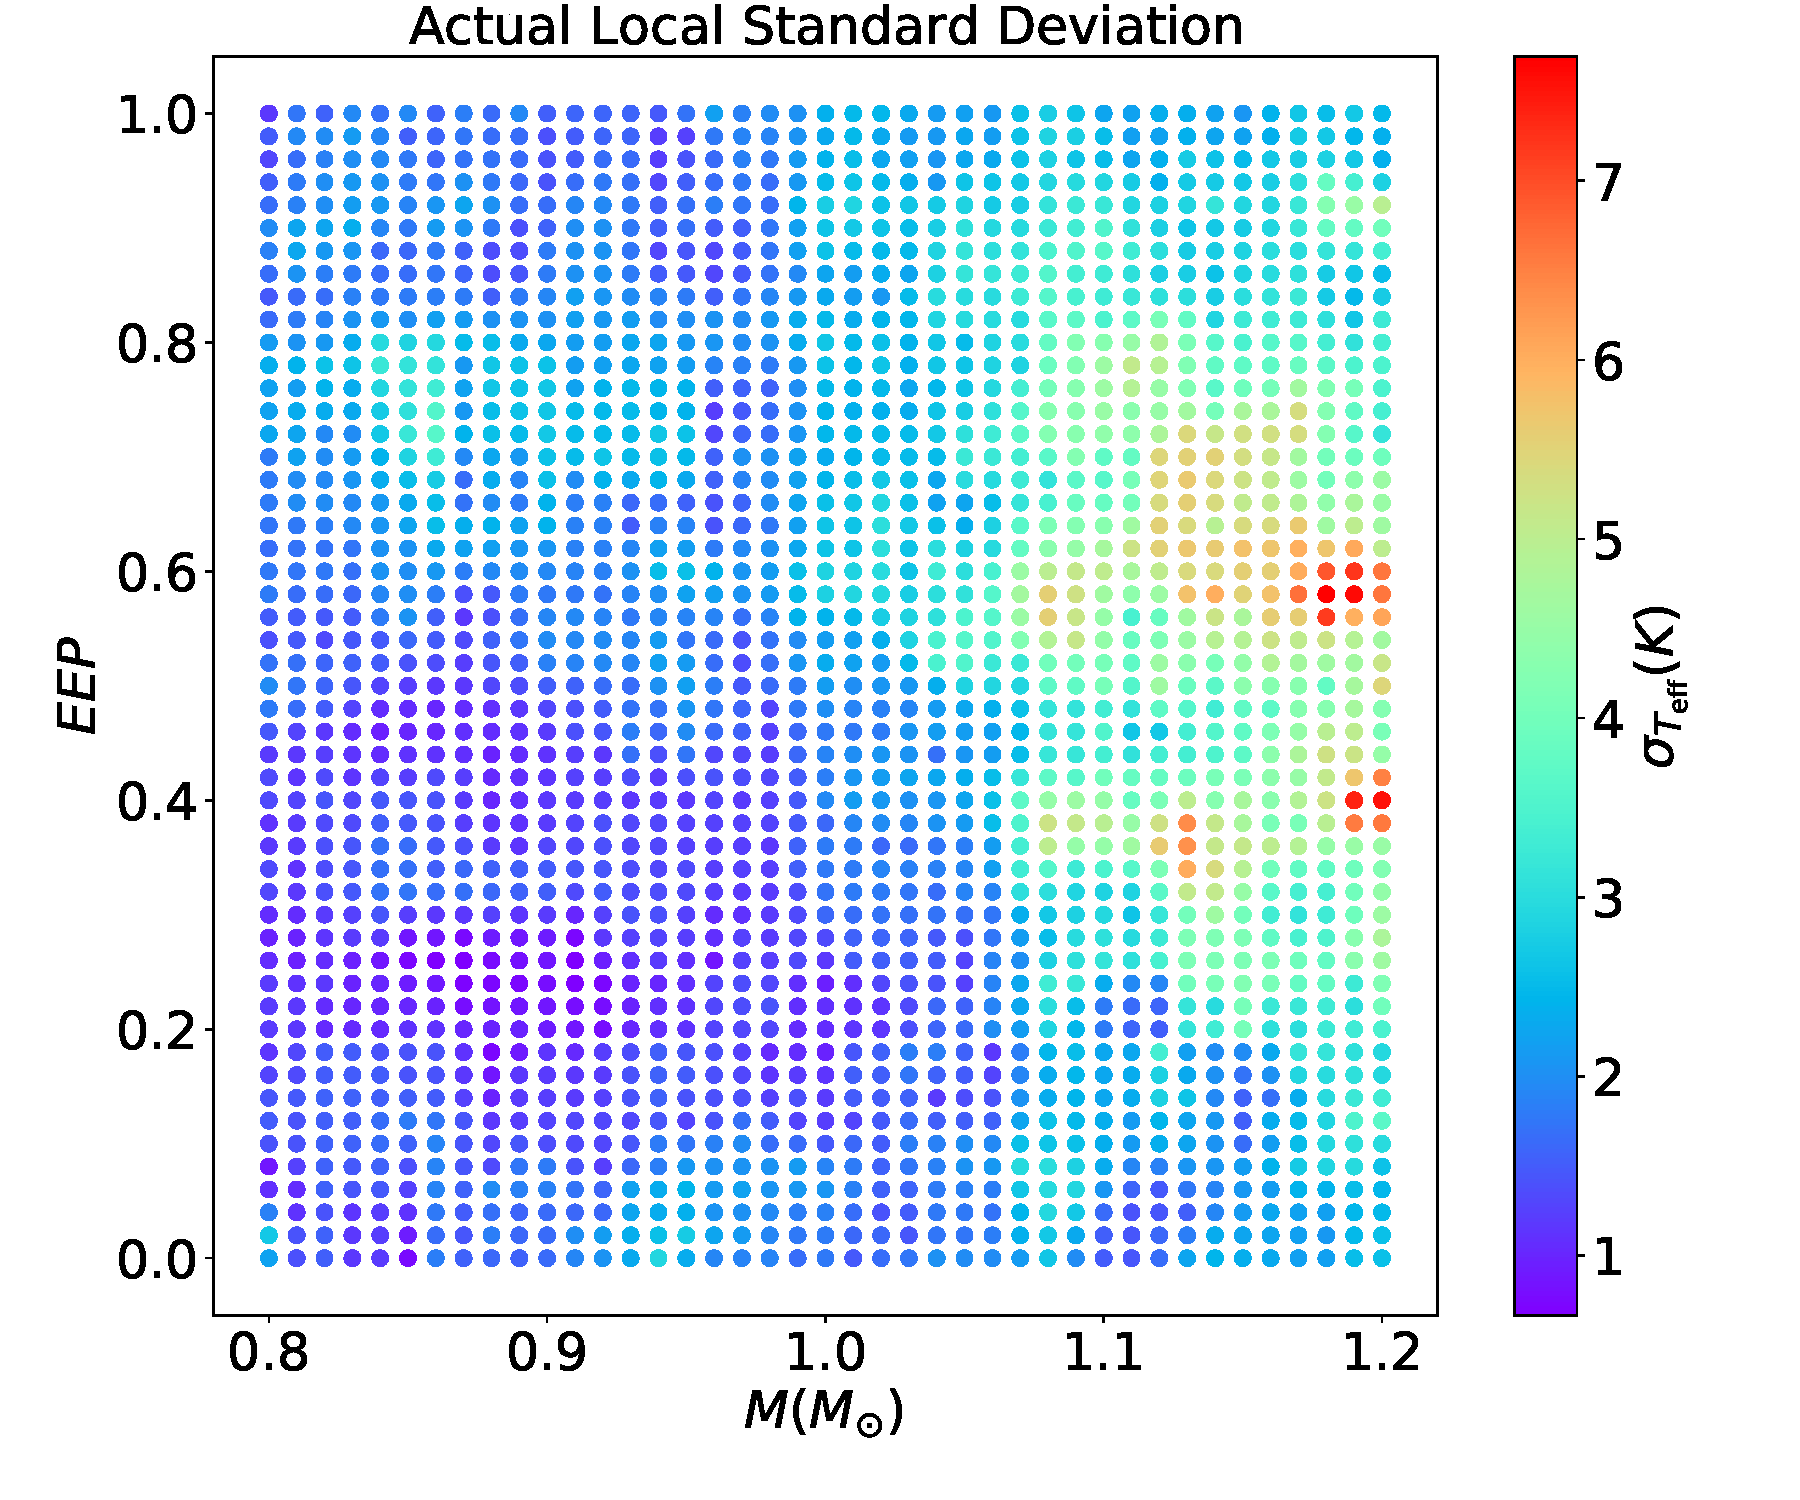
\includegraphics[width=1.0\columnwidth]{5d_sys_teff.pdf}
	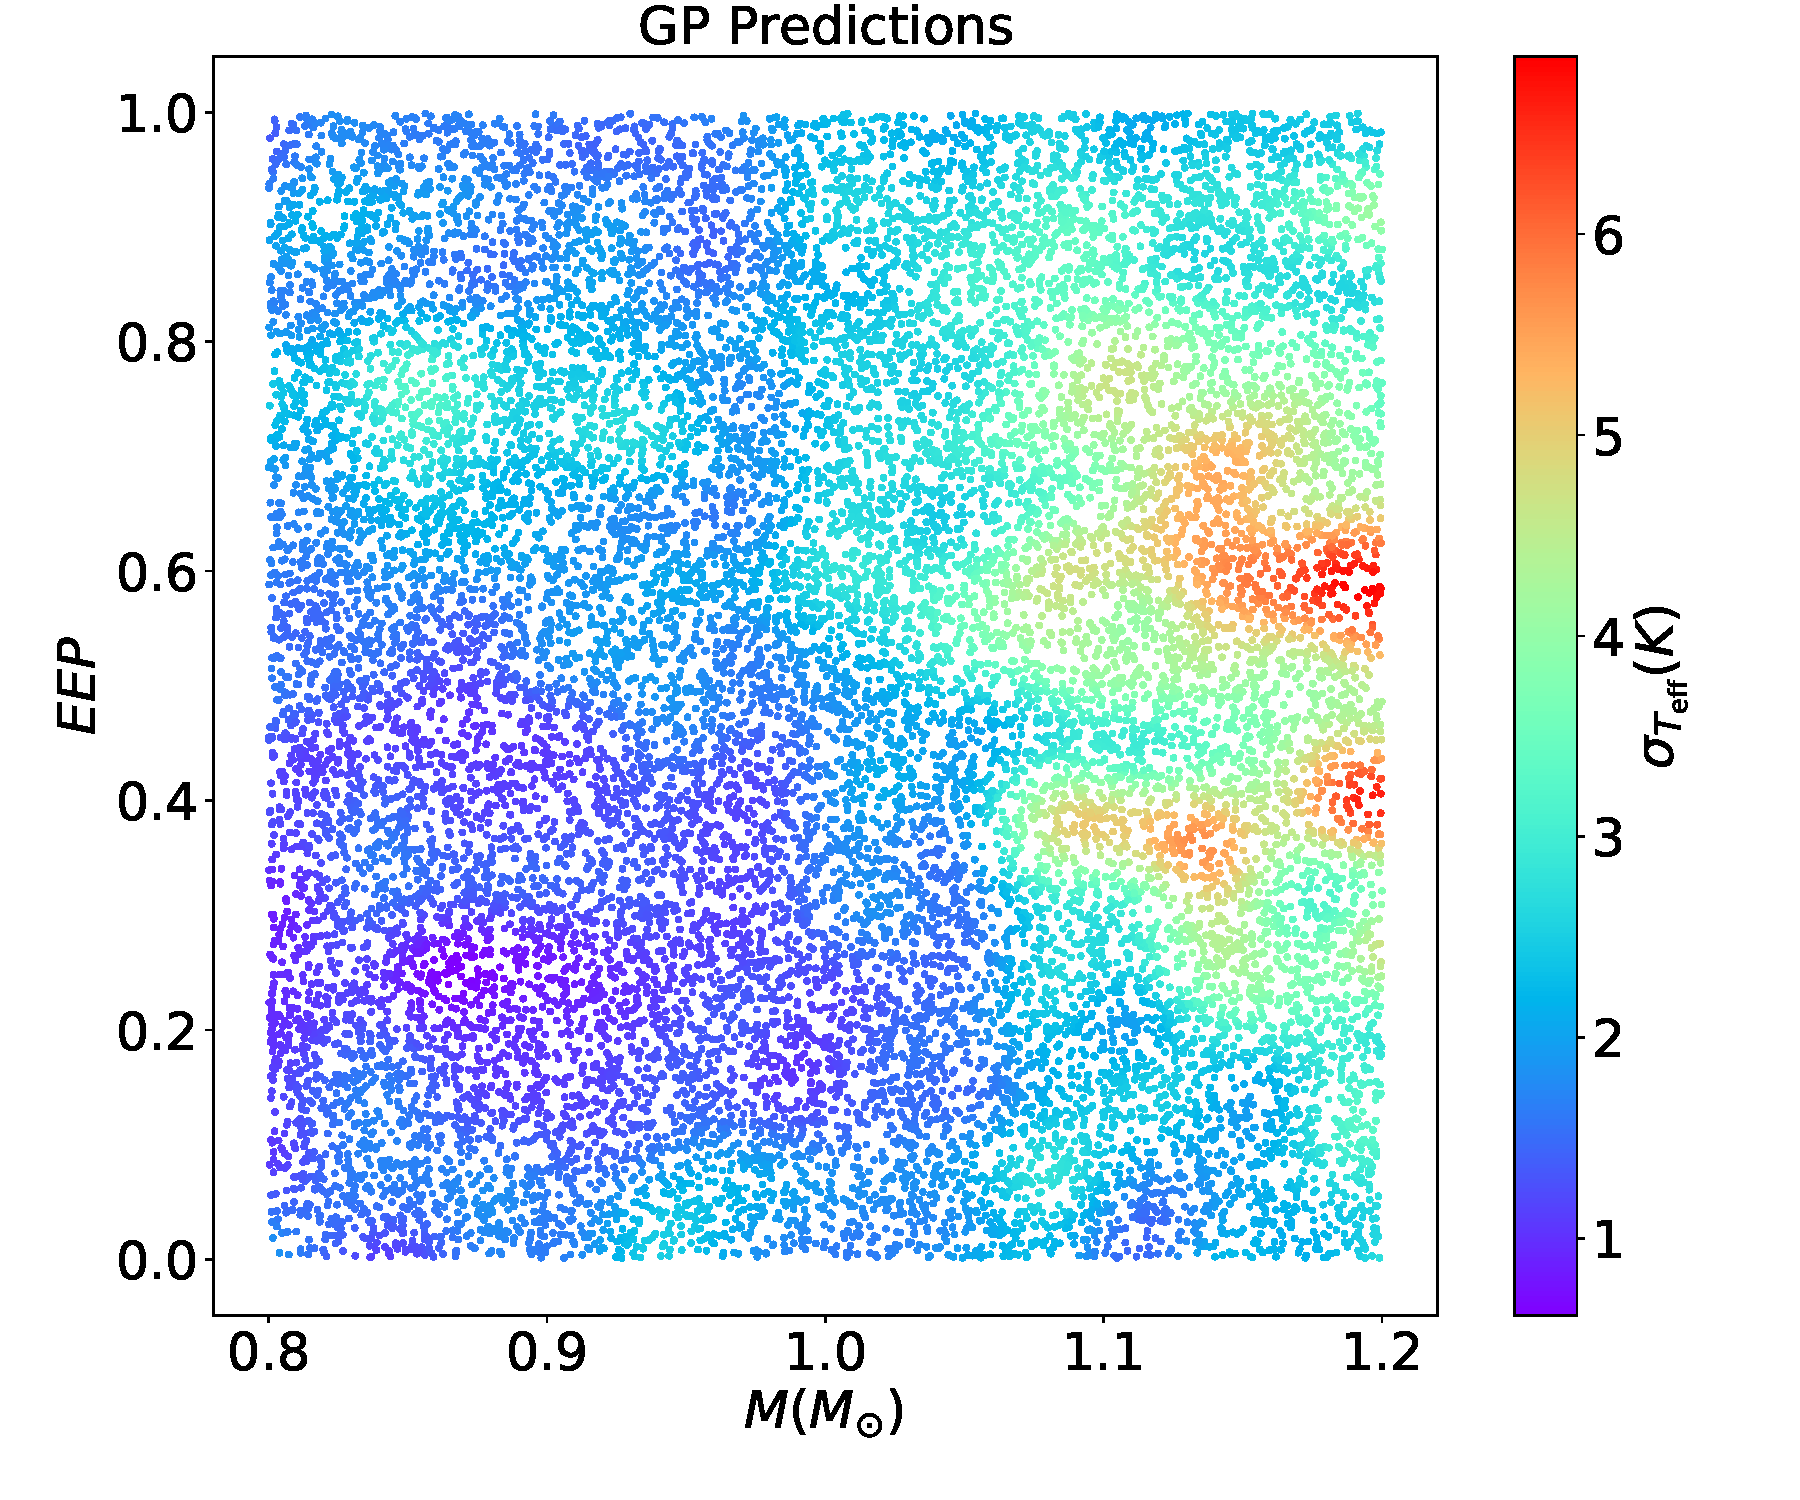
\includegraphics[width=1.0\columnwidth]{5d_sys_effective_T_std_predictions.pdf}
    \caption{Local standard deviations of testing errors for $T_{\rm eff}$ on the $M -- EEP$ diagram ([Fe/H]$_{\rm init}$ = 0.0). } 
  \label{fig:5d_sys_teff}
\end{figure}

We train and validate GP-SYS model for each output parameter. In Figure \ref{fig:5d_sys_teff}, we demonstrate the actual $\sigma_{T_{\rm eff}}$ and the GP-trained $\sigma_{T_{\rm eff}}$ for $\rm [Fe/H]_{init}$ on the $M-EEP$ diagram.  As it can be seen that, GP well reproduces the $\sigma_{T_{\rm eff}}$ distributions. Validation errors are in a range of $\pm1K$ and the average residual is only 0.15K. We summary the average residuals for all five output parameter in Table \ref{tab:sys}.

\begin{table}
	\centering
	\caption{Residual of GP models for systematic uncertainty}
	\label{tab:sys}
	\begin{tabular}{lc}
		\hline
		GP output& Average Residual \\
		\hline
		$\sigma_{T_{\rm eff}}$  (K) & 0.15 \\
		$\sigma_{\log g}$  ($10^{-3}$dex)   & 0.08 \\
		$\sigma_{R}$ ($10^{-3}R_{\odot}$)   & 0.2 \\
		$\sigma_{\rm [Fe/H]_{\rm surf}}$ ($10^{-3}$dex) & 0.09 \\
		$\sigma_{\tau}$ ($10^{-2}$ Gyr)  & 0.2\\
		%$\sigma_{\Delta\nu} (\mu Hz)$ & 0.01\\
		  \hline
	\end{tabular}
\end{table}


\section{Augmentation of the MESA Grid}

We have obtained GP-Grid models for predicting observable outputs and GP-SYS models for estimating systematical uncertainty. 
In Figure~\ref{fig:5d_augmentation}, we demonstrate GP-trained Kiel diagrams across four input demissions, i.e., $M$, [Fe/H]$_{\rm init}$, $Y_{\rm init}$, and $\alpha_{\rm MLT}$. Compared with the sparse MESA grid, GP models turn it into a non-sparse model set. {\bf some discussions about the FIgure.}

\begin{figure*}
	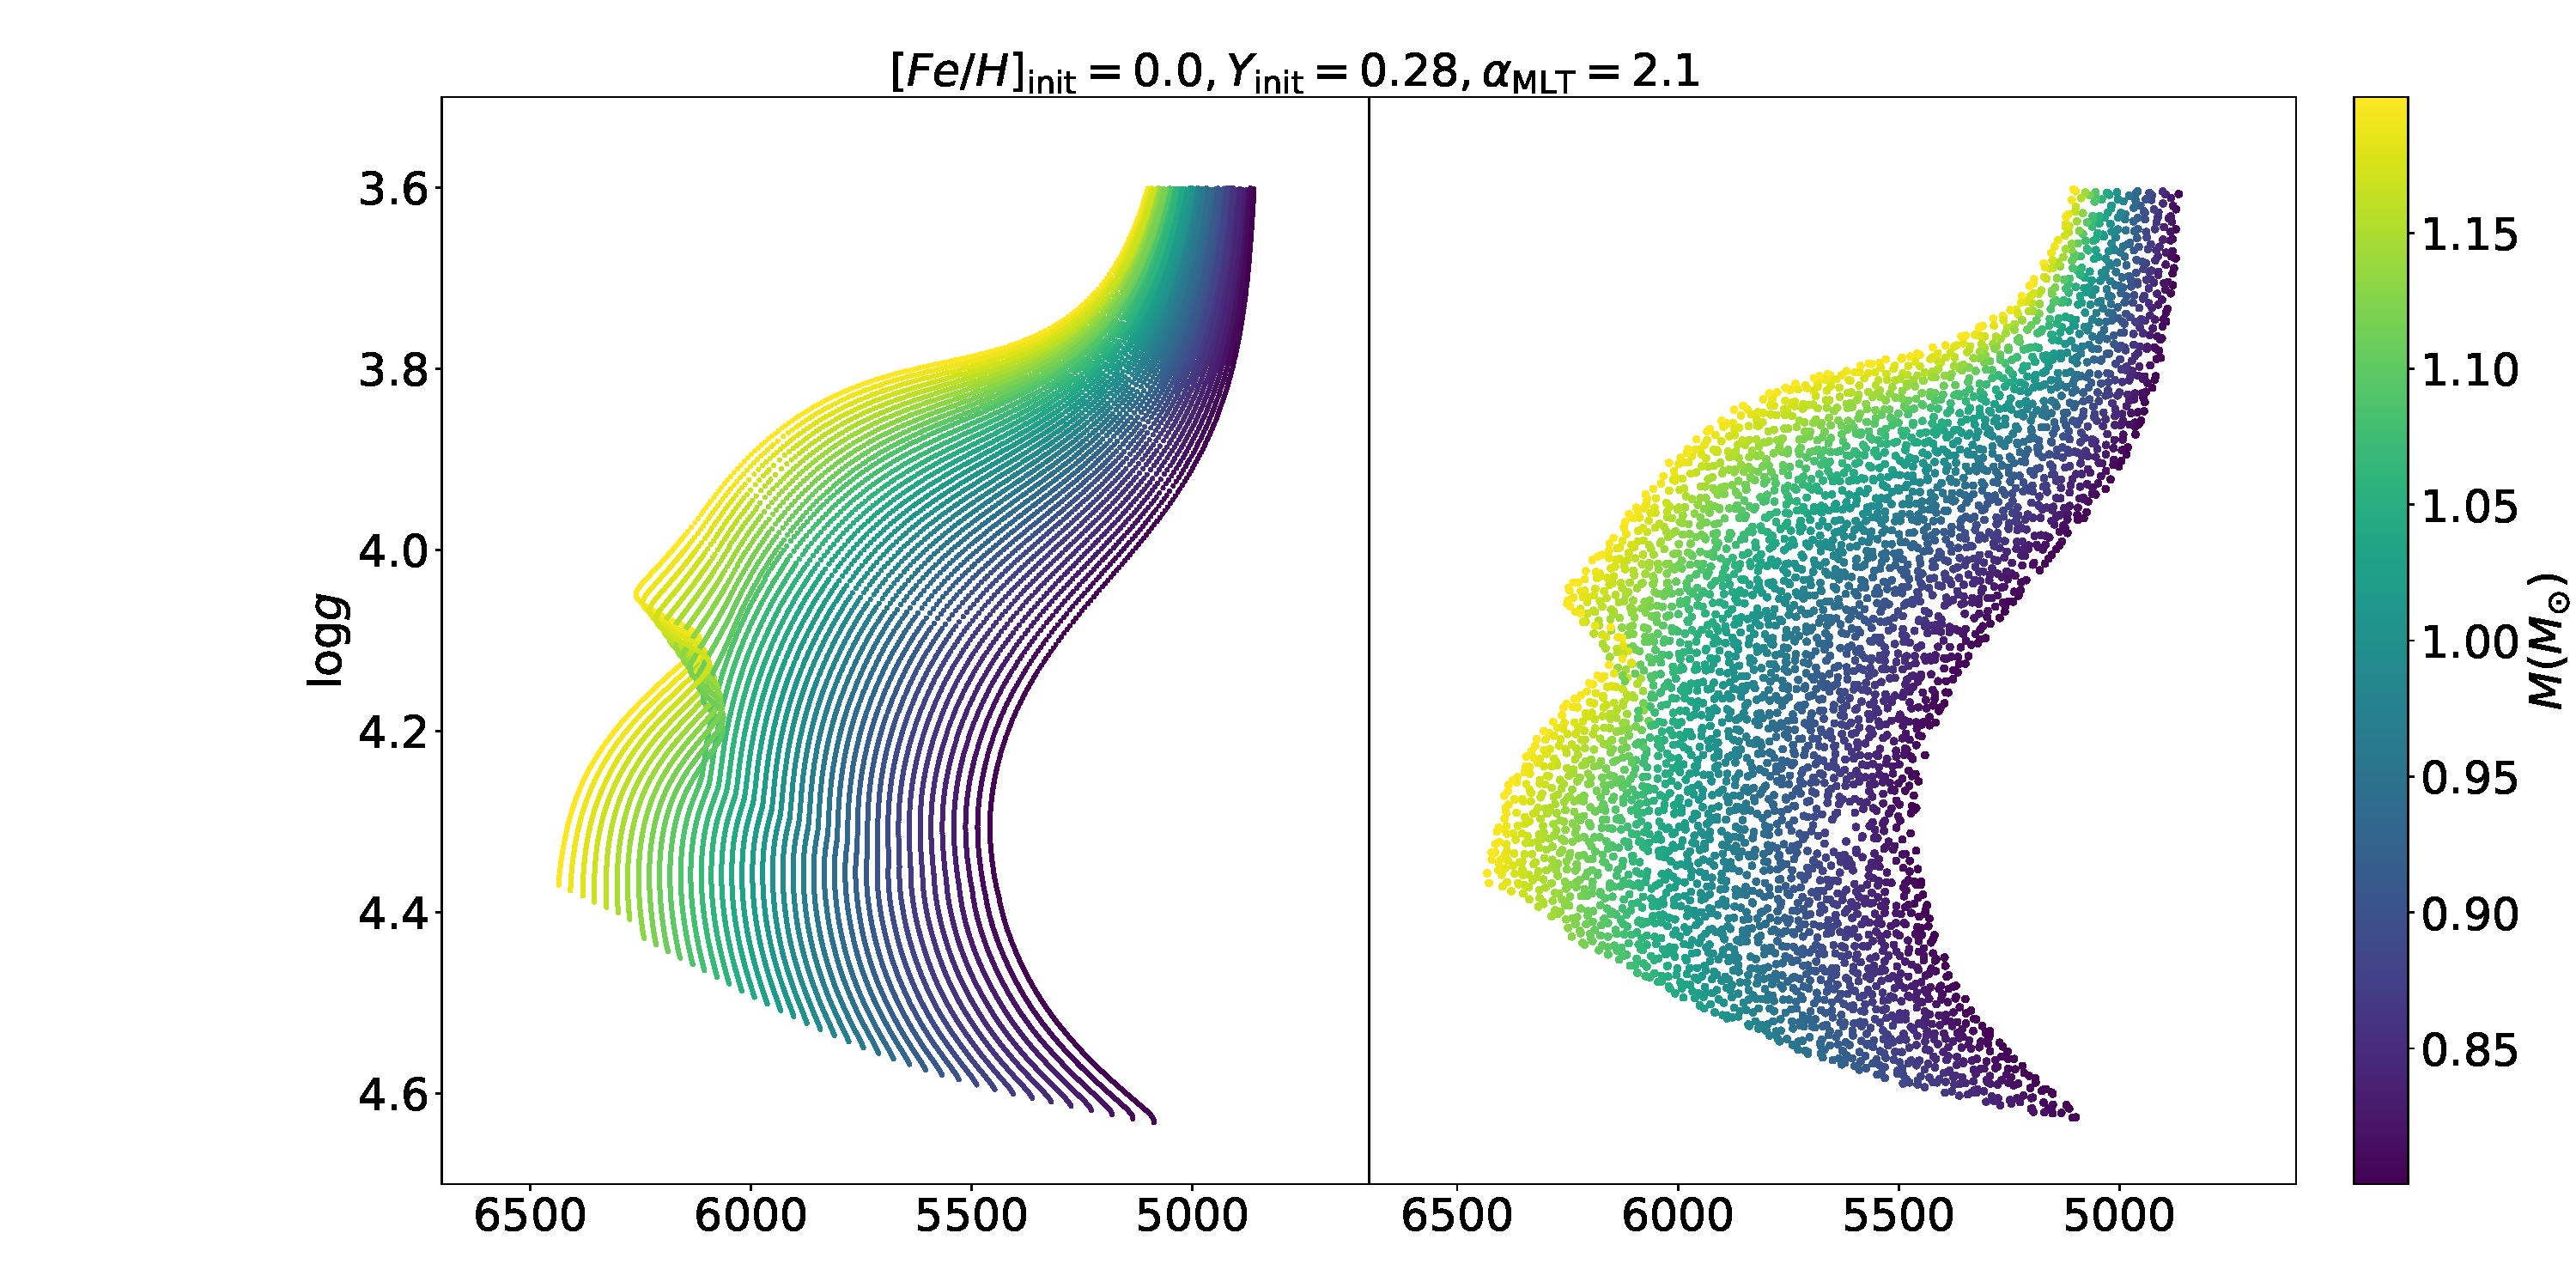
\includegraphics[width=1.2\columnwidth]{5d-au-mass.pdf}
	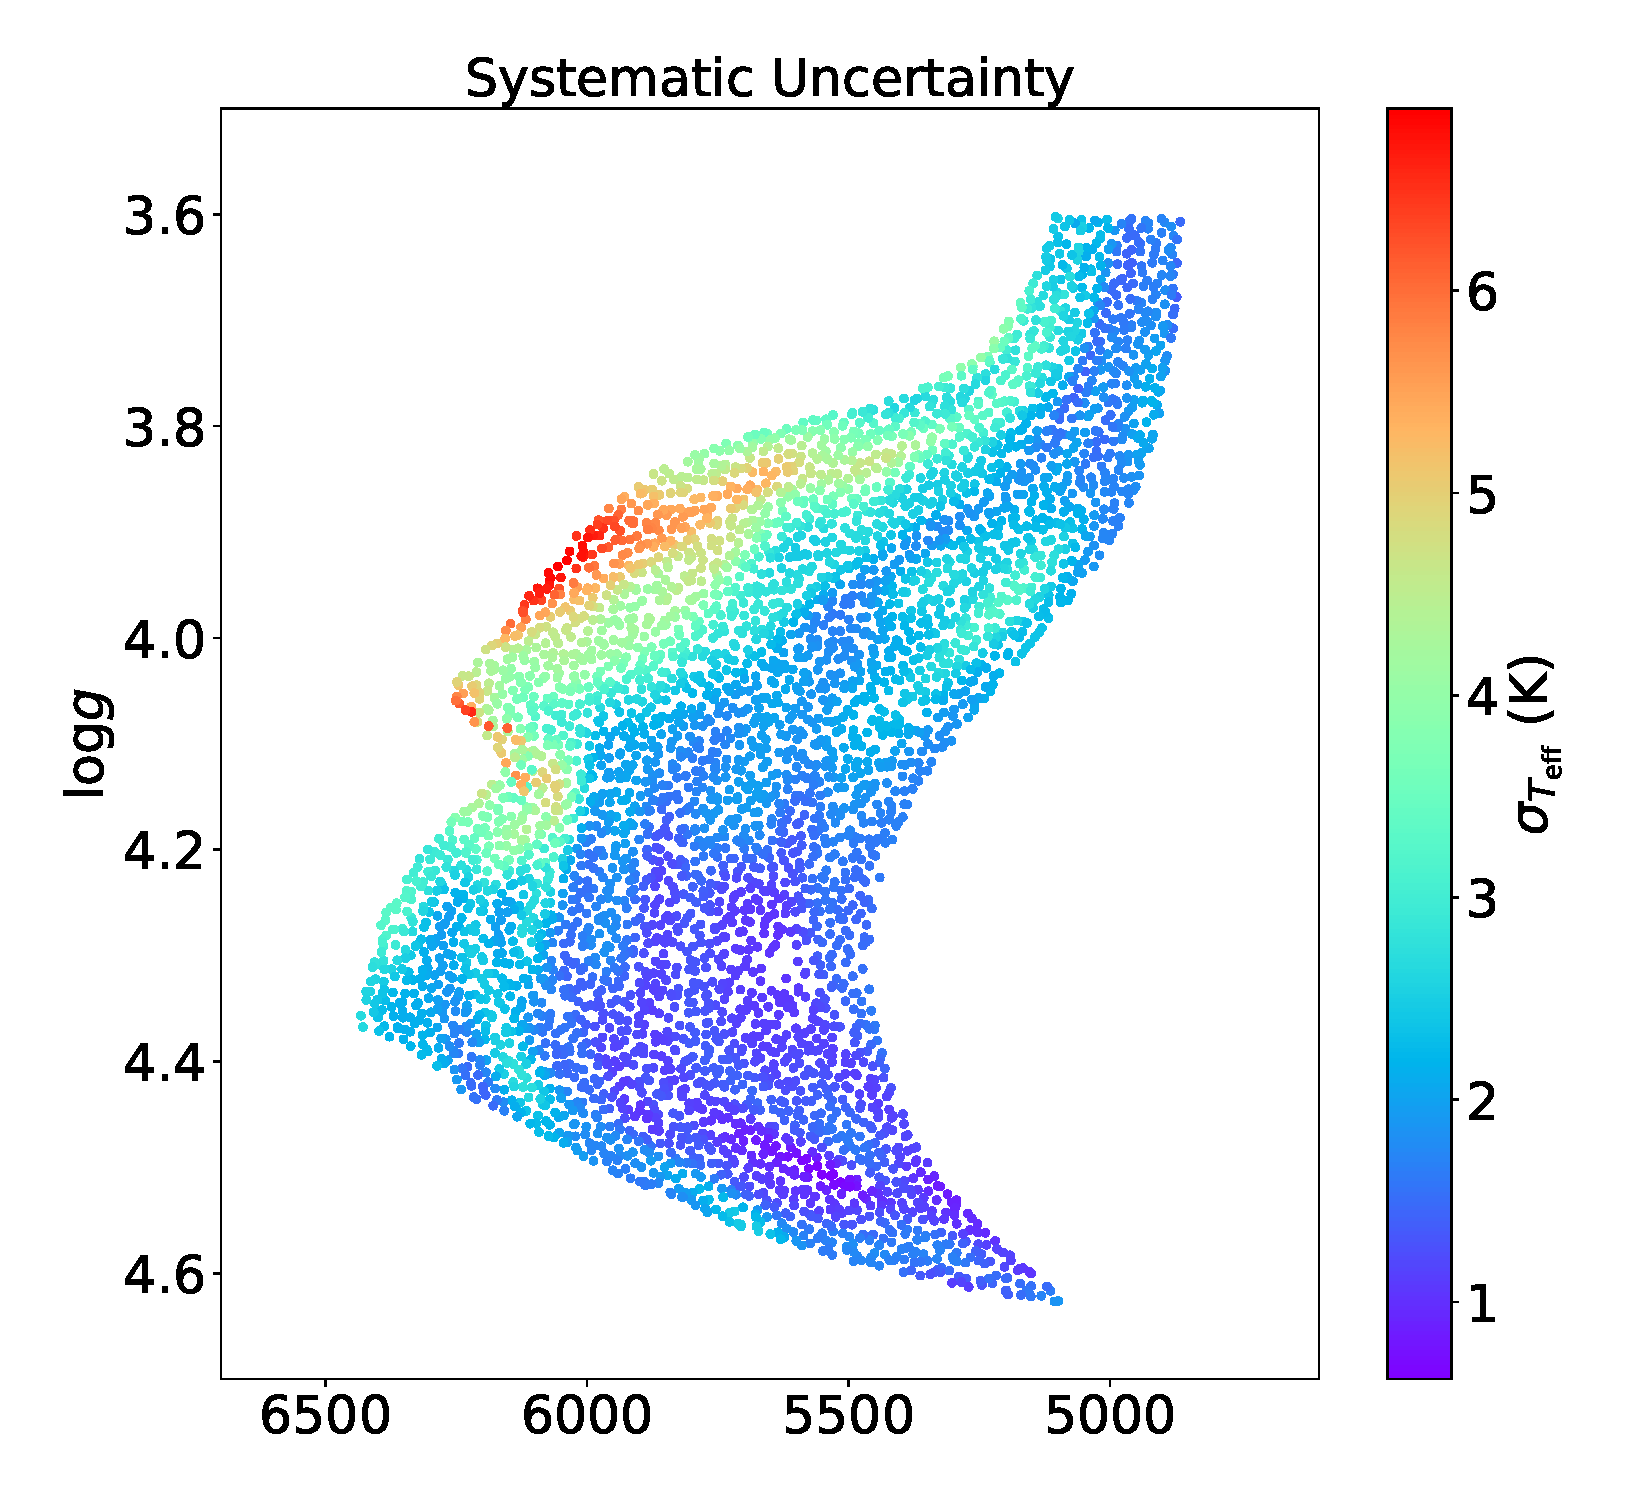
\includegraphics[width=0.65\columnwidth]{5d-au-mass-sys.pdf}
	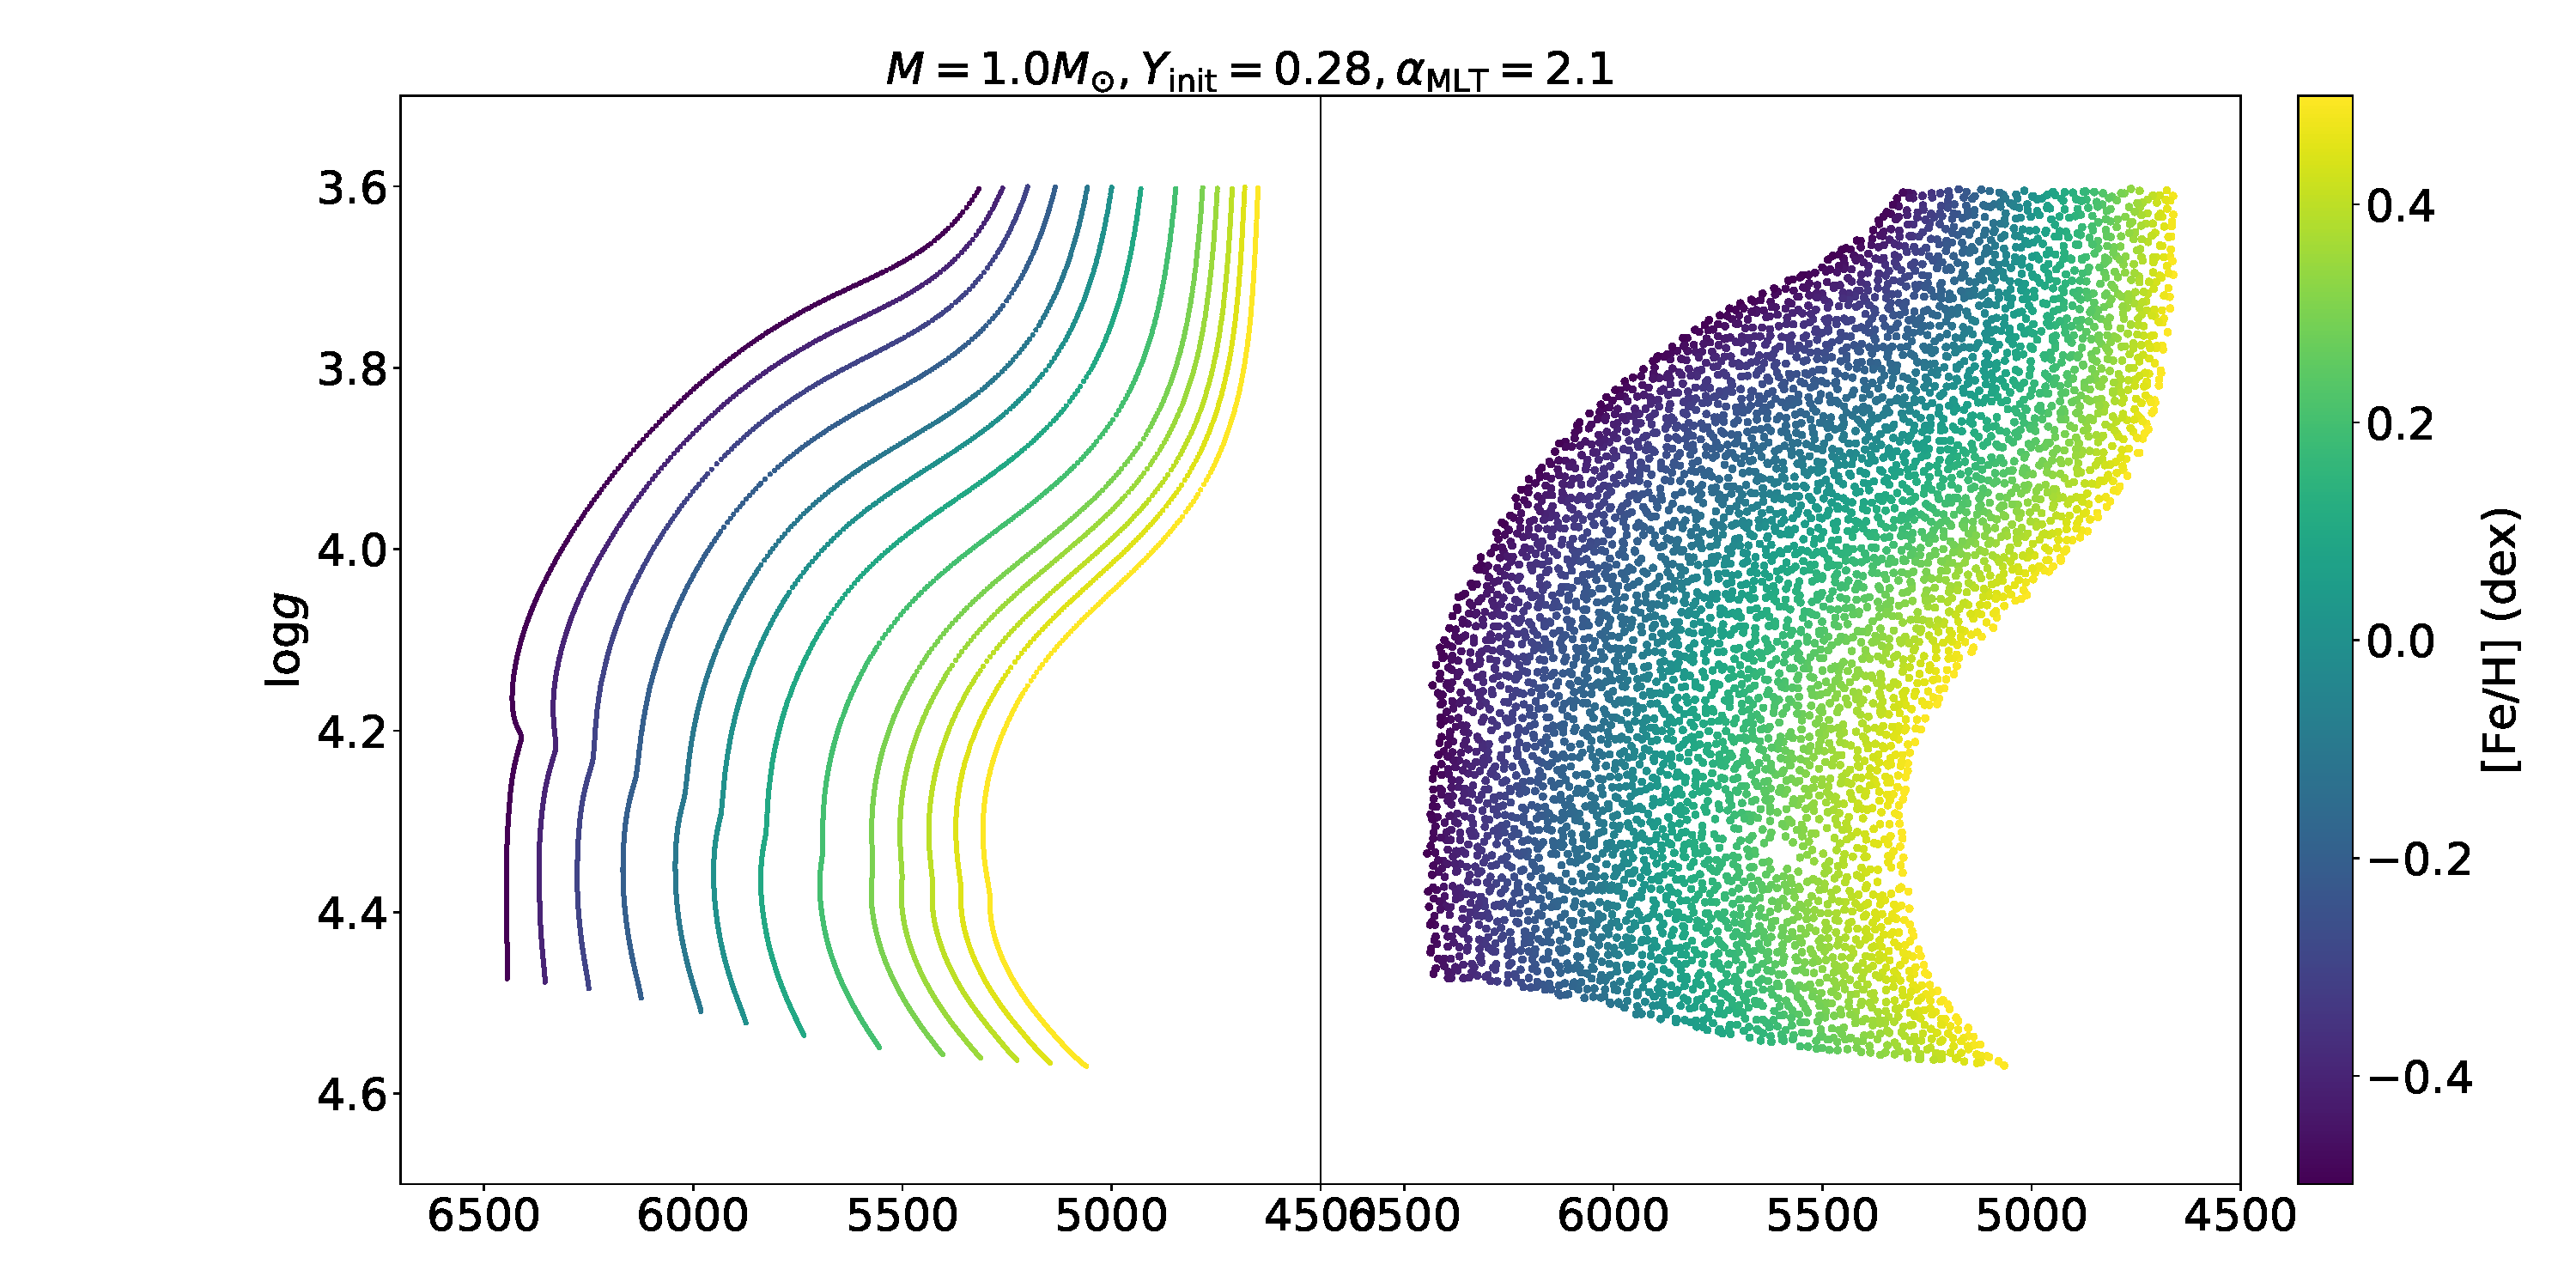
\includegraphics[width=1.2\columnwidth]{5d-au-feh.pdf}
	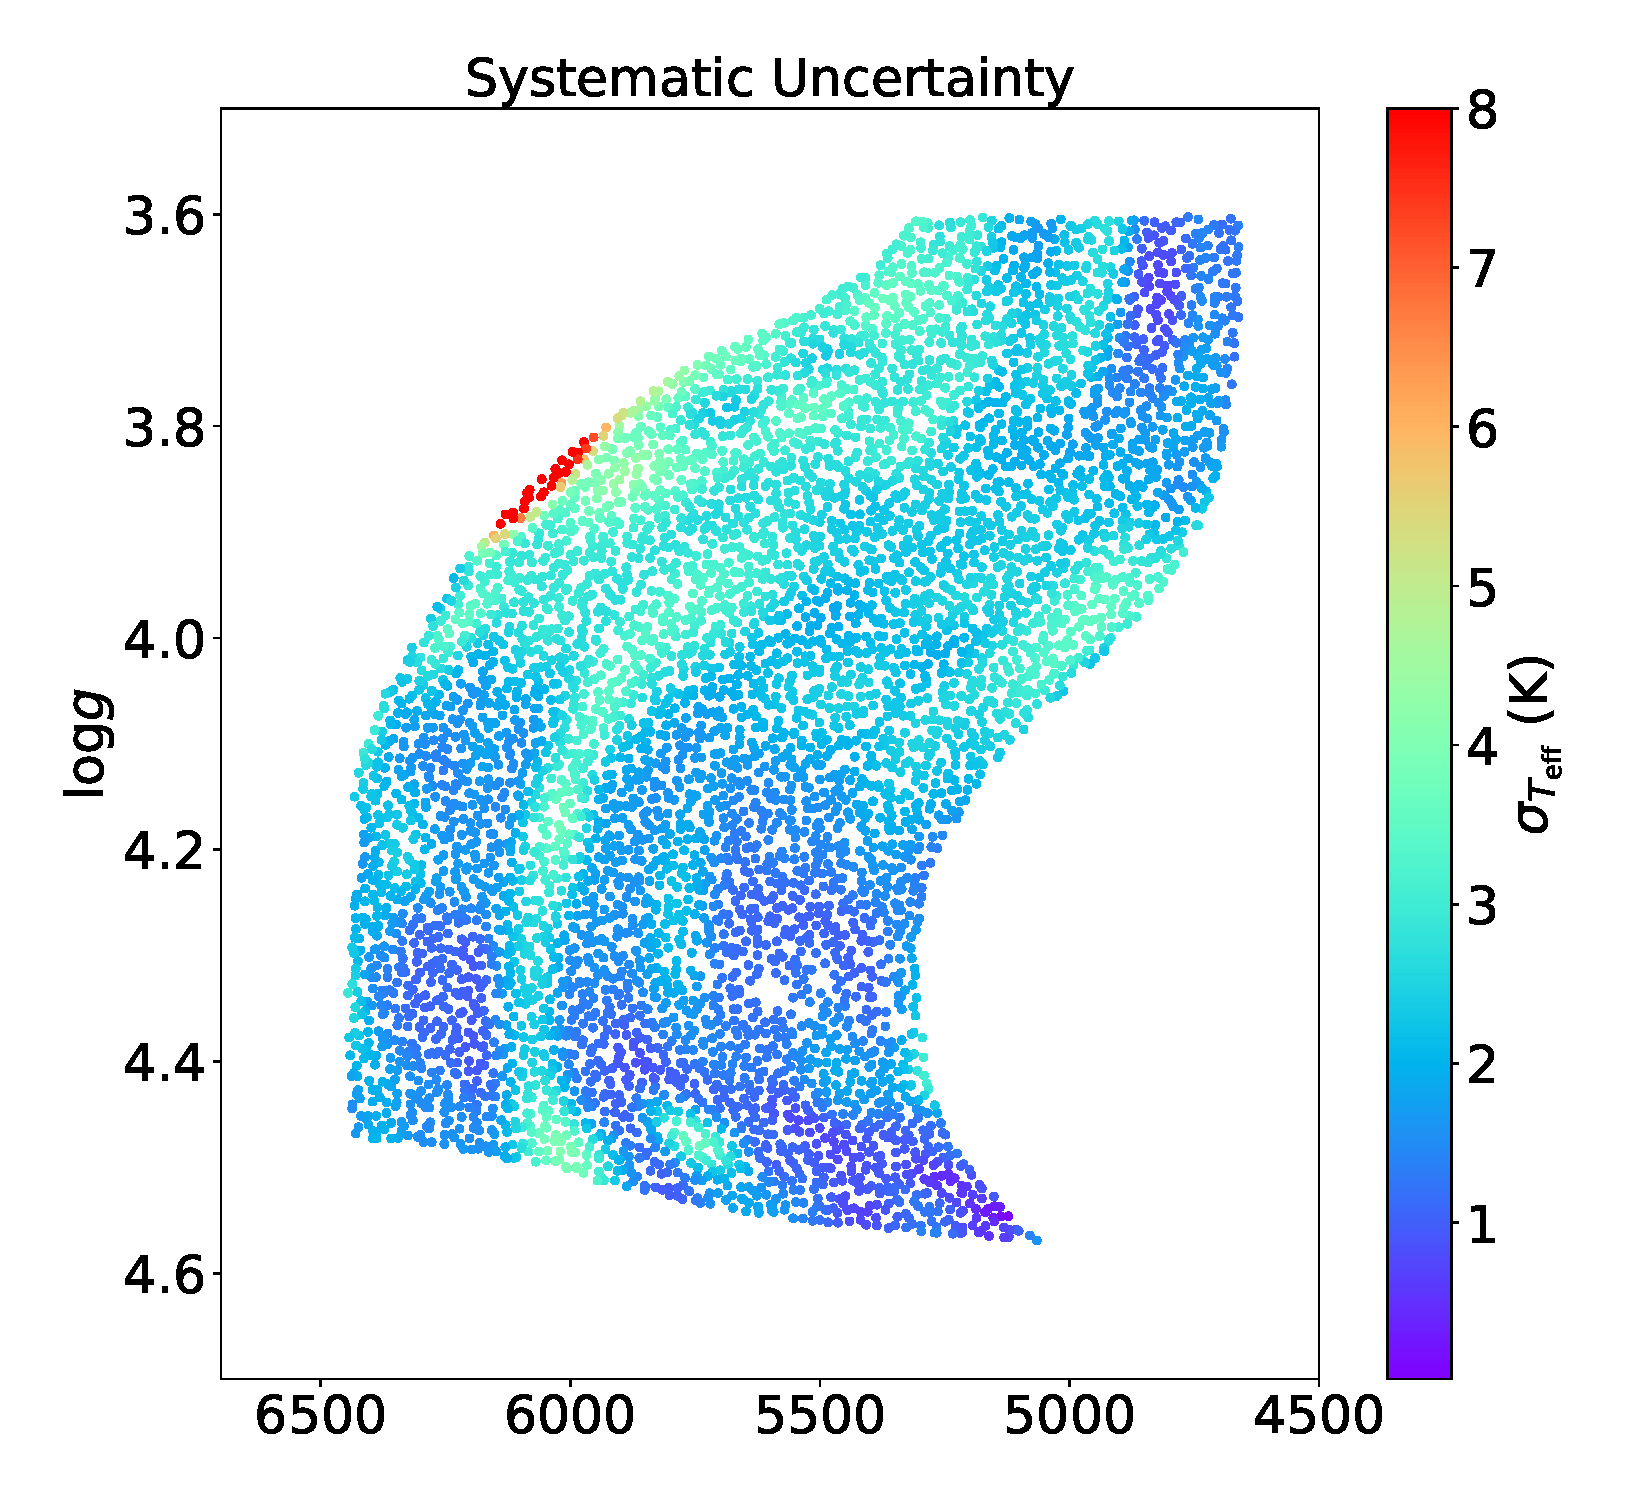
\includegraphics[width=0.65\columnwidth]{5d-au-feh-sys.pdf}
	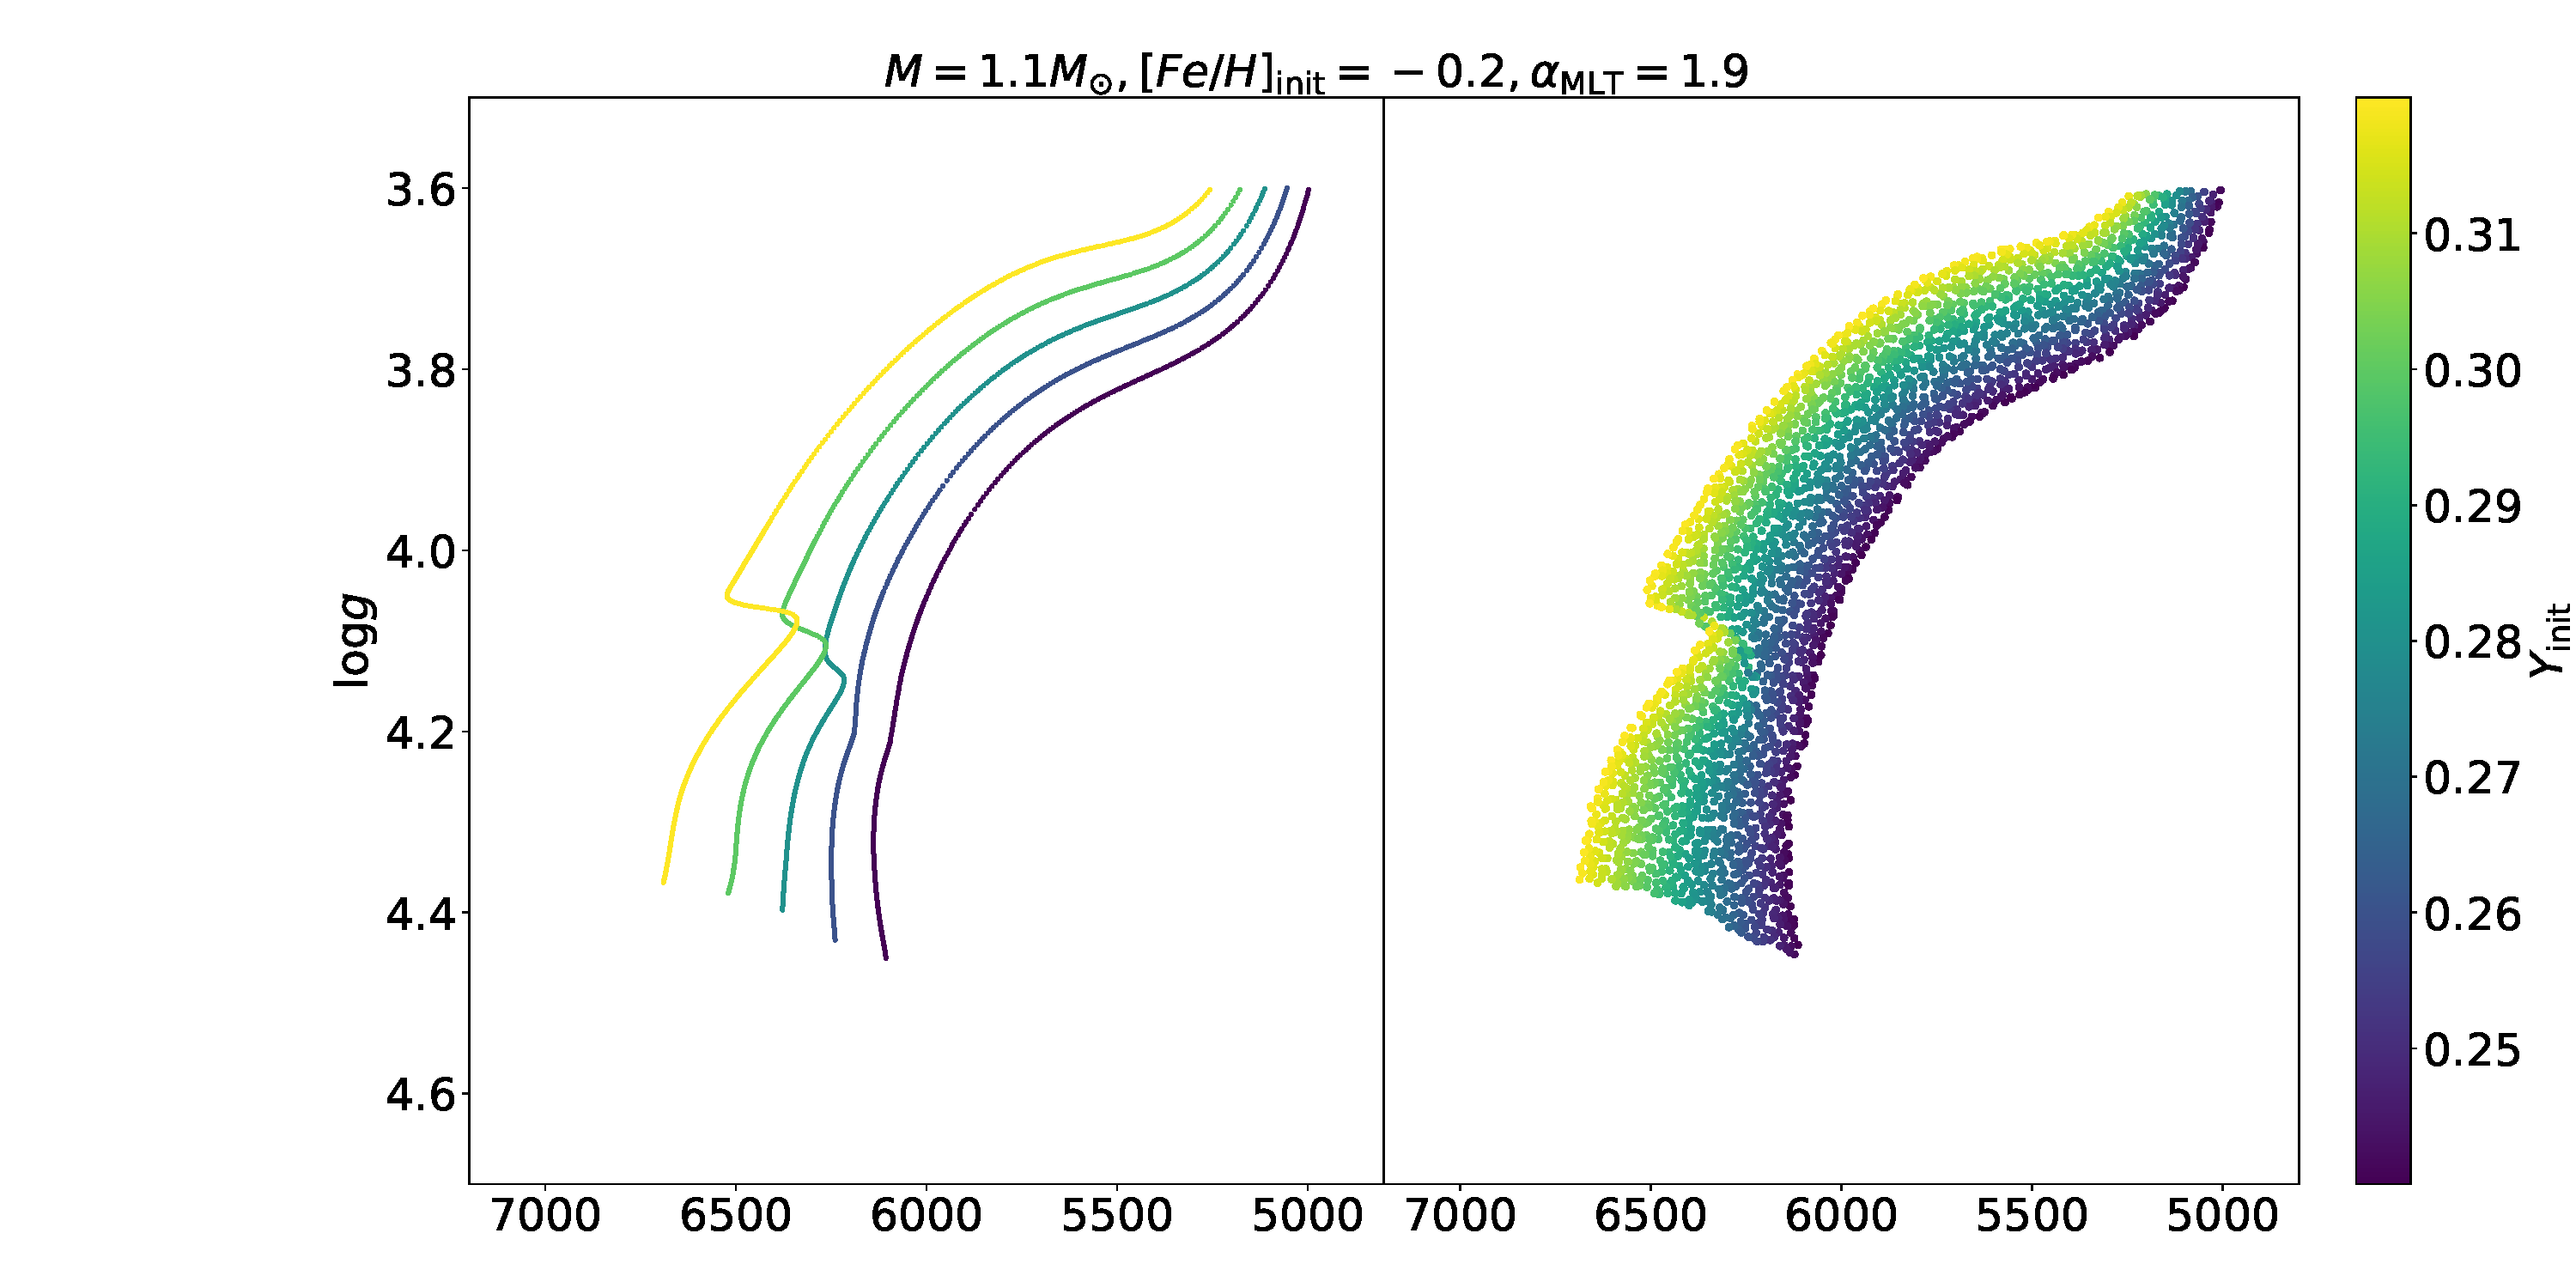
\includegraphics[width=1.2\columnwidth]{5d-au-y.pdf}
	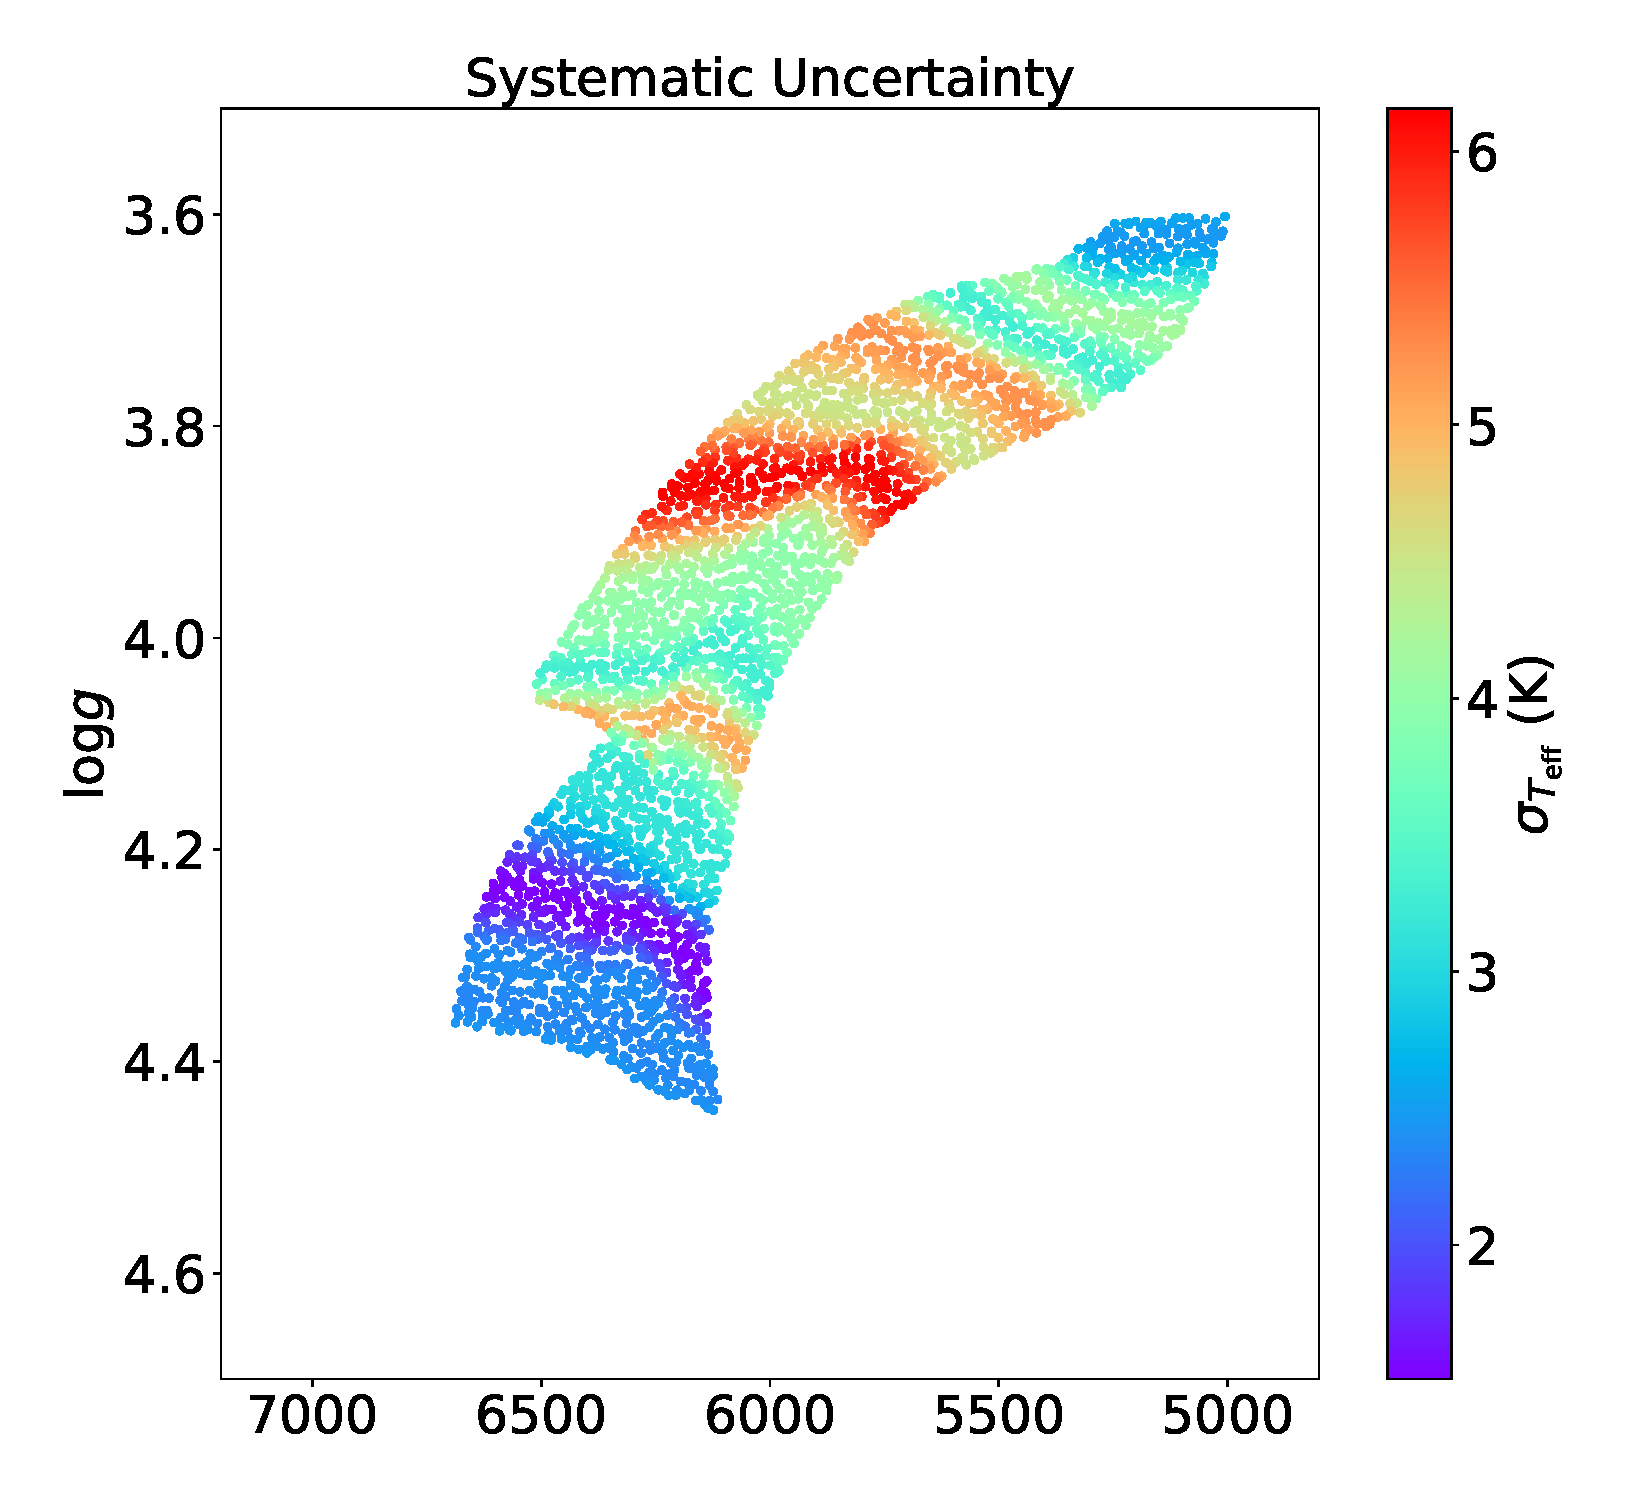
\includegraphics[width=0.65\columnwidth]{5d-au-y-sys.pdf}
	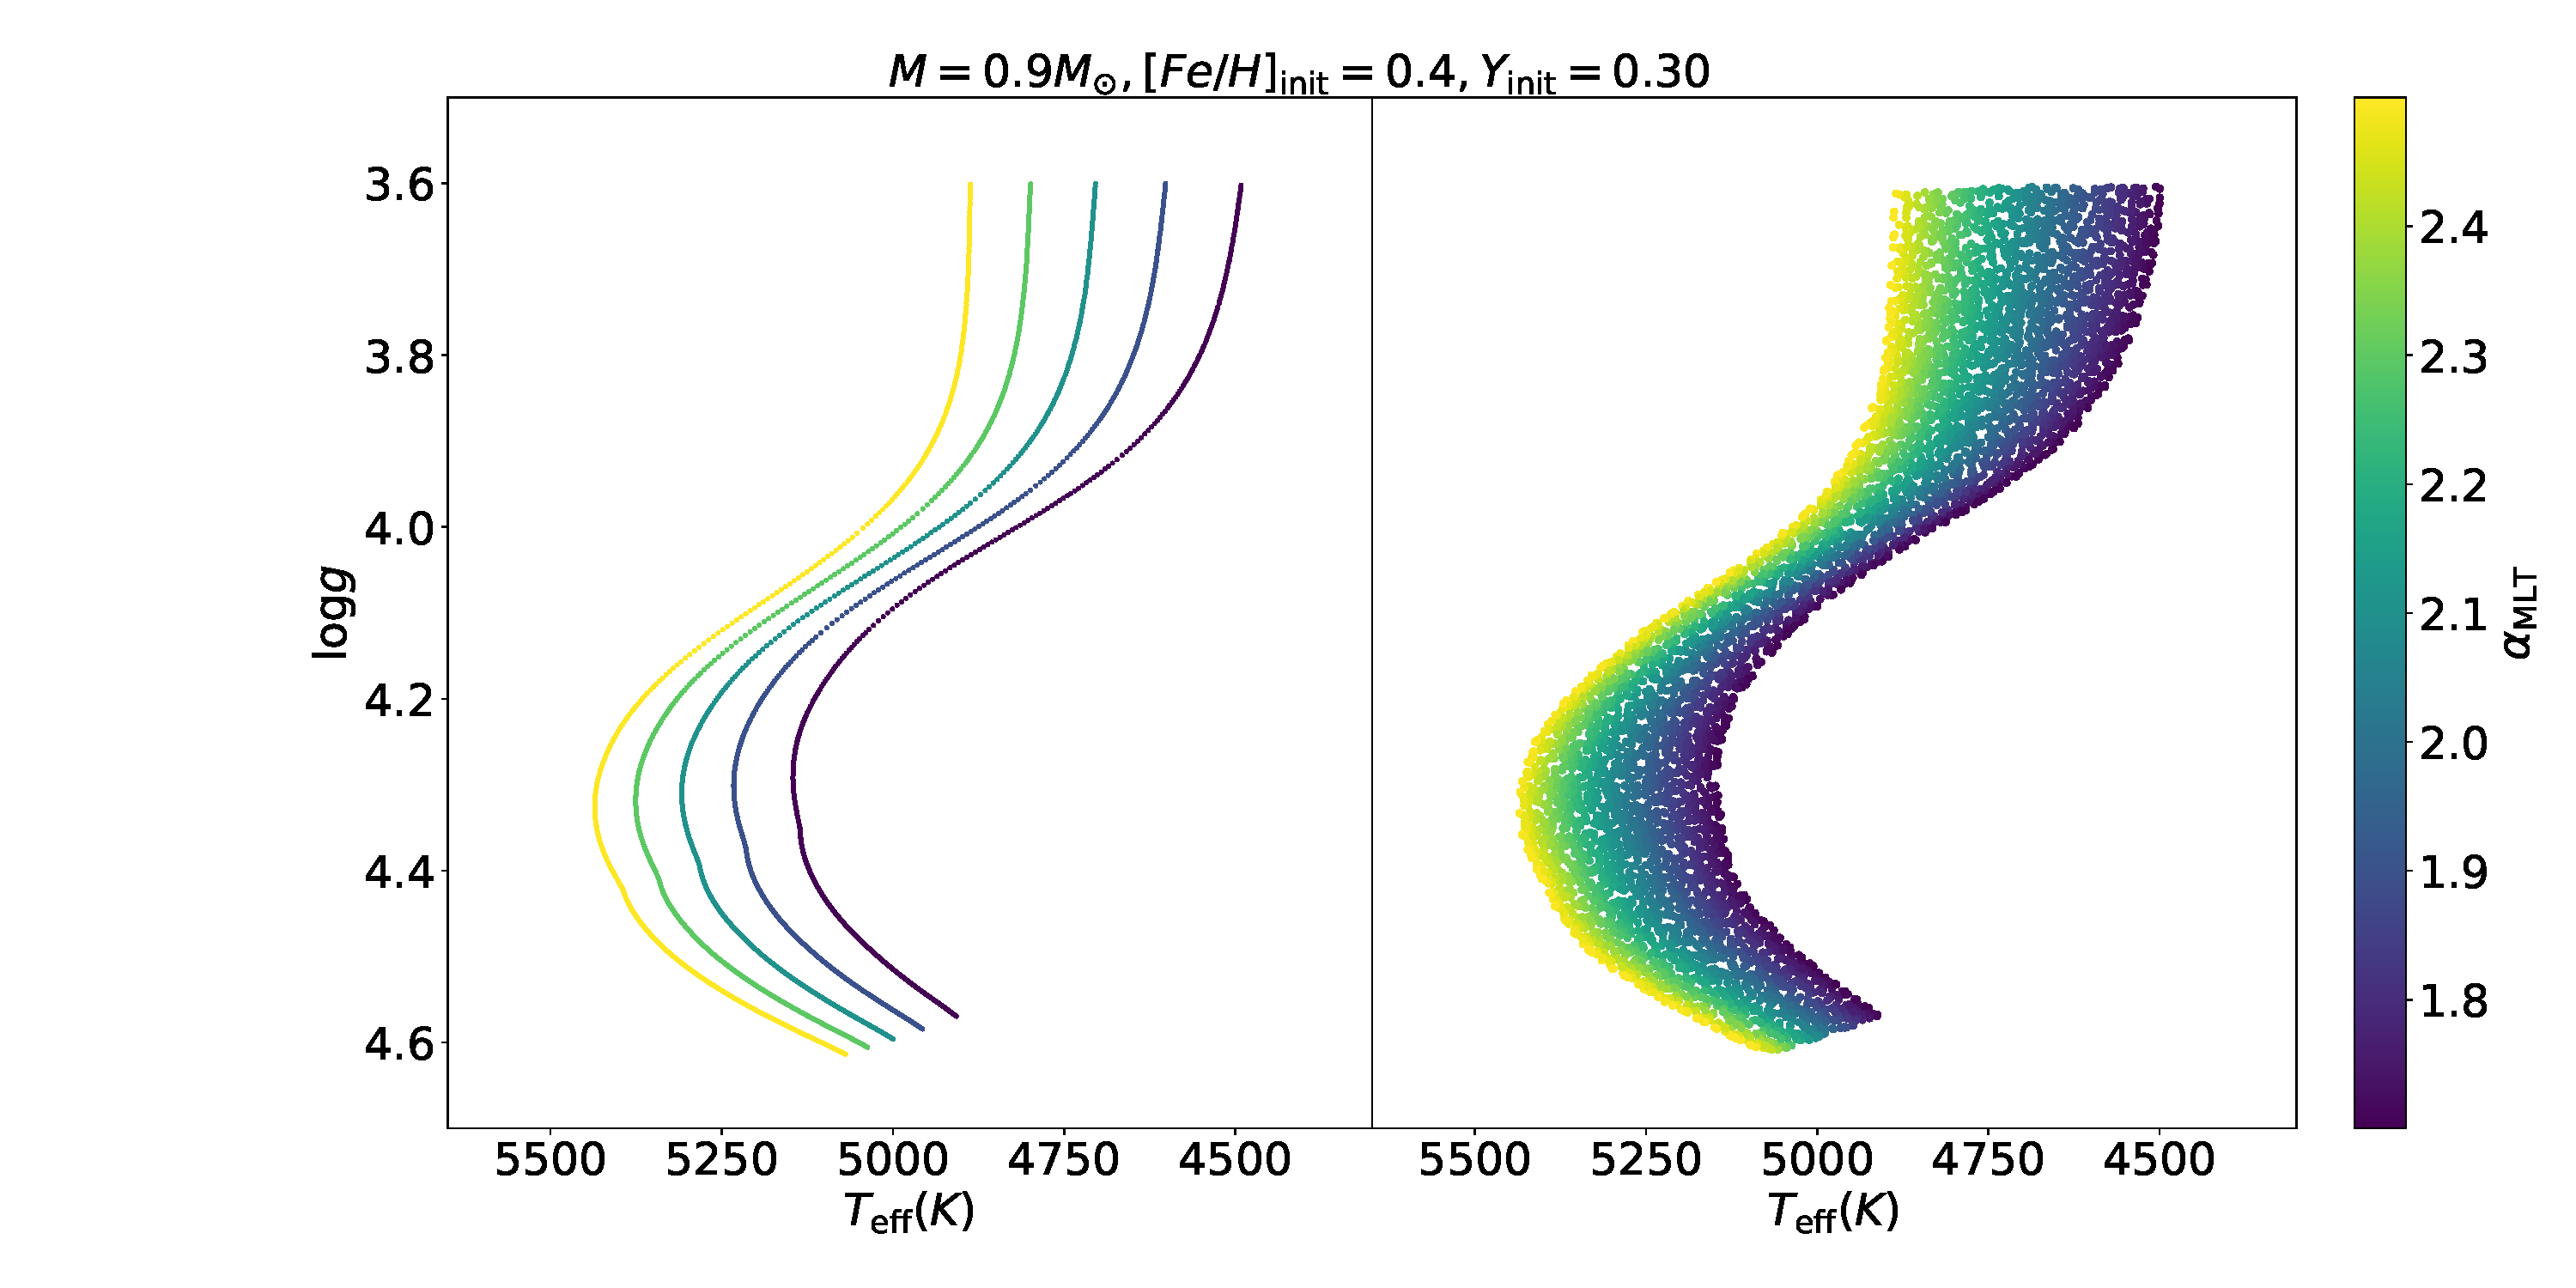
\includegraphics[width=1.2\columnwidth]{5d-au-alpha.pdf}
	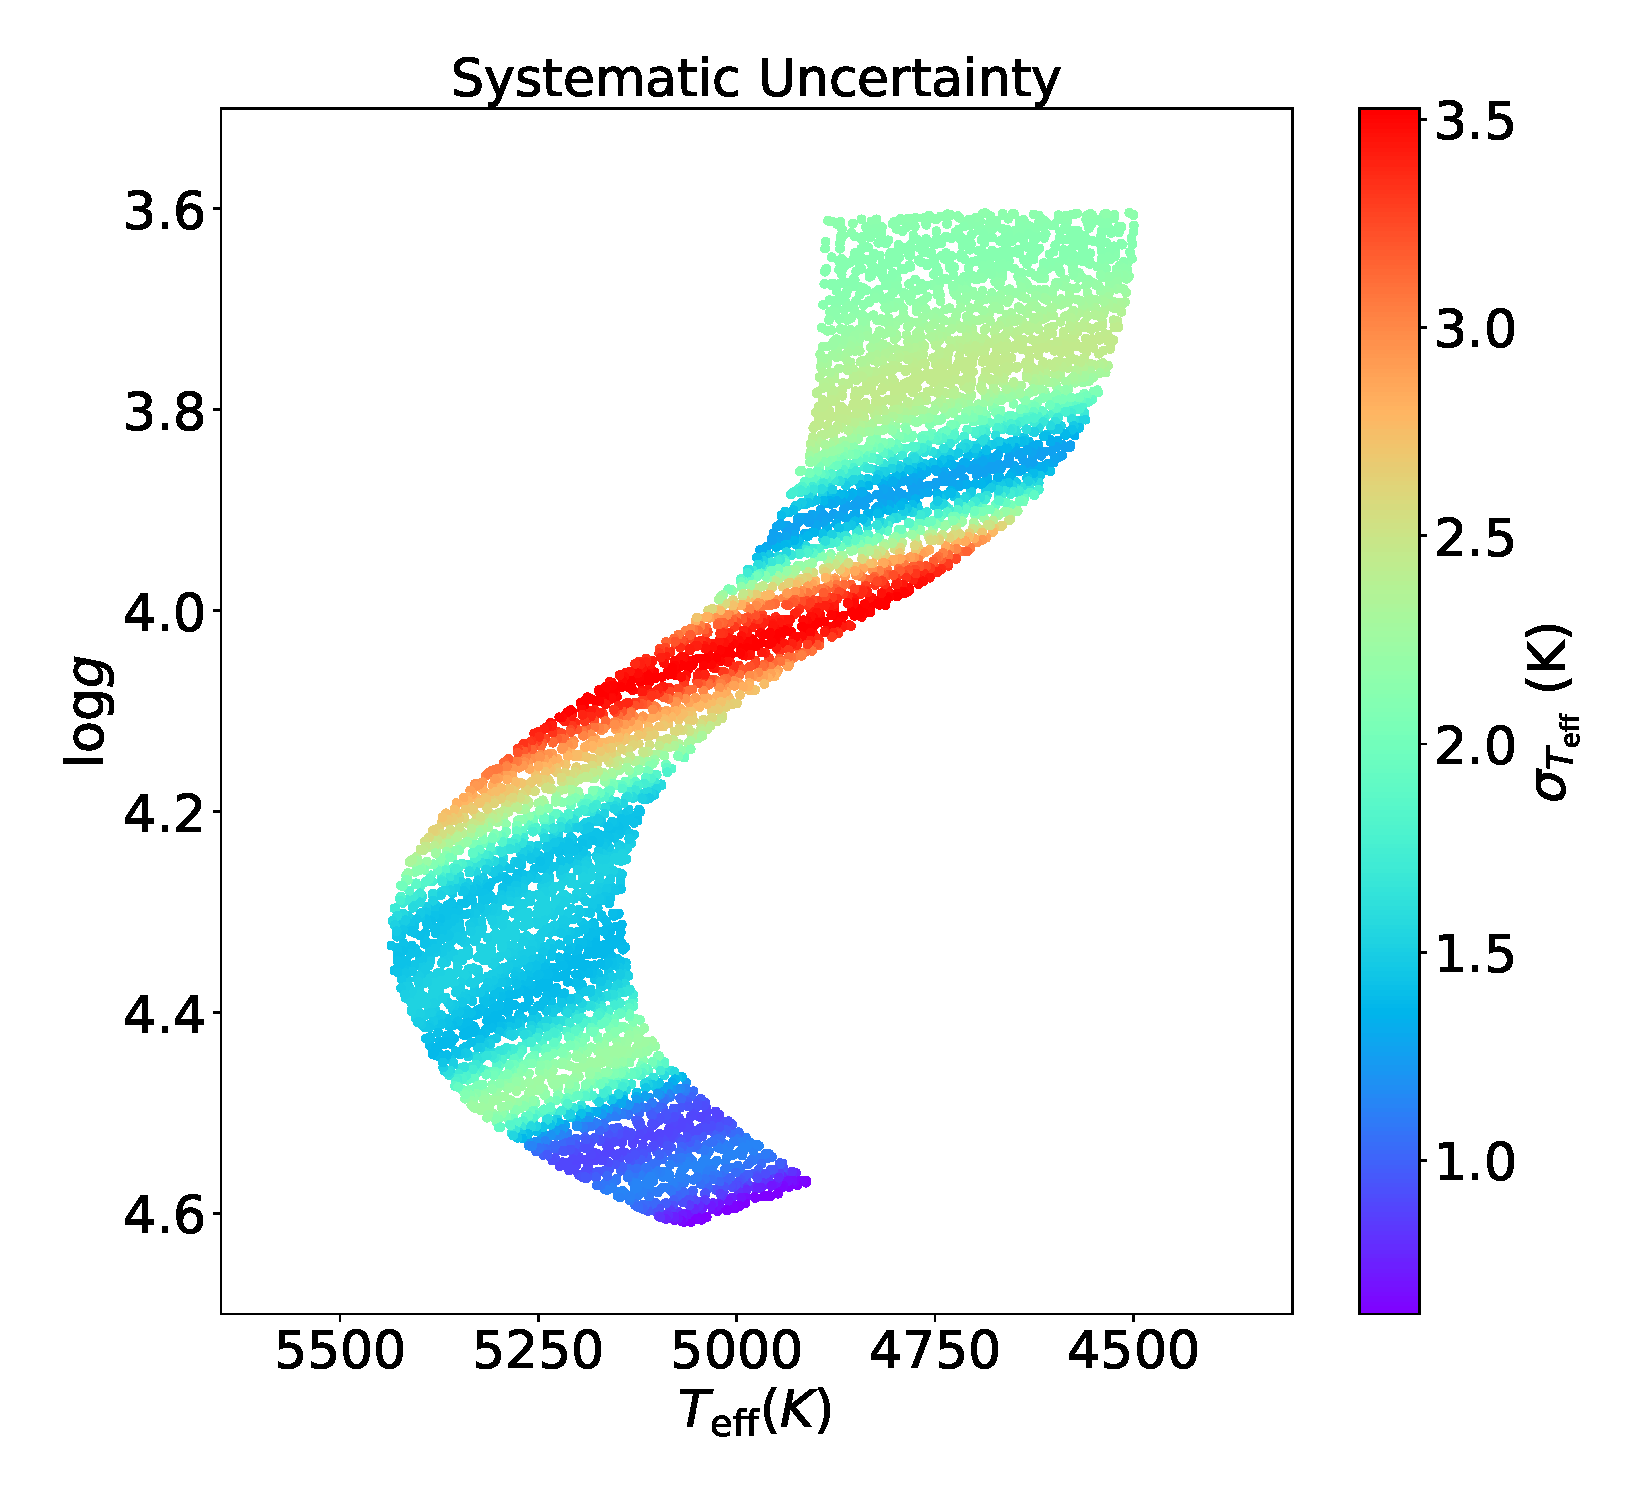
\includegraphics[width=0.65\columnwidth]{5d-au-alpha-sys.pdf}
    \caption{GP-trained models and their systematic uncertainties across four demissions on the Kiel diagram.} 
  \label{fig:5d_augmentation}
\end{figure*}

We augment the MESA model grid and turn it into a continuously sampled model set which contents 5,000,000 model data points. We randomly sample GP model inputs with flat distributions, predict observable outputs with GP-Grid models and systematic uncertainties with GP-SYS models. The model set includes five fundamental inputs ($M$, $EEP$, [Fe/H]$_{\rm init}$, $Y_{\rm init}$, and $\alpha_{\rm MLT}$), five outputs, ($T_{\rm eff}$, $\log g$,  $R$,  [Fe/H]$_{\rm surf}$, and  $\tau$), and five systematic uncertainties ($\sigma_{T_{\rm eff}}$, $\sigma_{\log g}$,  $\sigma_{R}$,  $\sigma_{\rm [Fe/H]_{\rm surf}}$, and $\sigma_{\tau}$). This model set can be downloaded at \url{a-place-for-data}. We listed 10 models in Table XXX as examples. 

\subsection{Modelling fake stars with GP-trained models}

We lastly test the general performance of GP models by modelling 100 fake stars. Fake stars are randomly selected from the off-grid MESA models. We use four observables, i.e., $T_{\rm eff}$, $\log g$, $R$, and [Fe/H]$_{\rm surf}$, as input constraints. We applied typical observed uncertainty that is $\pm$50 K for $T_{\rm eff}$ (high-resolution spectroscopy), $\pm0.005$ for $\log g$ (seismology), $3\%$ for $R$ (seismology), and $\pm0.05$ for [Fe/H]$_{\rm surf}$ (high-resolution spectroscopy). 
%
To avoid edge effect, fakes stars are selected in the parameter ranges of 
$T_{\rm eff}$ = [4700K, 6800 K], $\log g$ = [3.7, 4.6], [Fe/H]$_{\rm surf}$ = [-0.35,0.35], $M$ = [0.85,1.15], $EEP$ = [0.05,0.95], $Y_{\rm init}$ = [0.25,0.31], and $\alpha_{\rm MLT}$ = [1.8,2.4]. 

Fitting method: 5$\sigma$ cut - MLE. discuss Figure 7. 

Discuss figure 8

\begin{figure}
	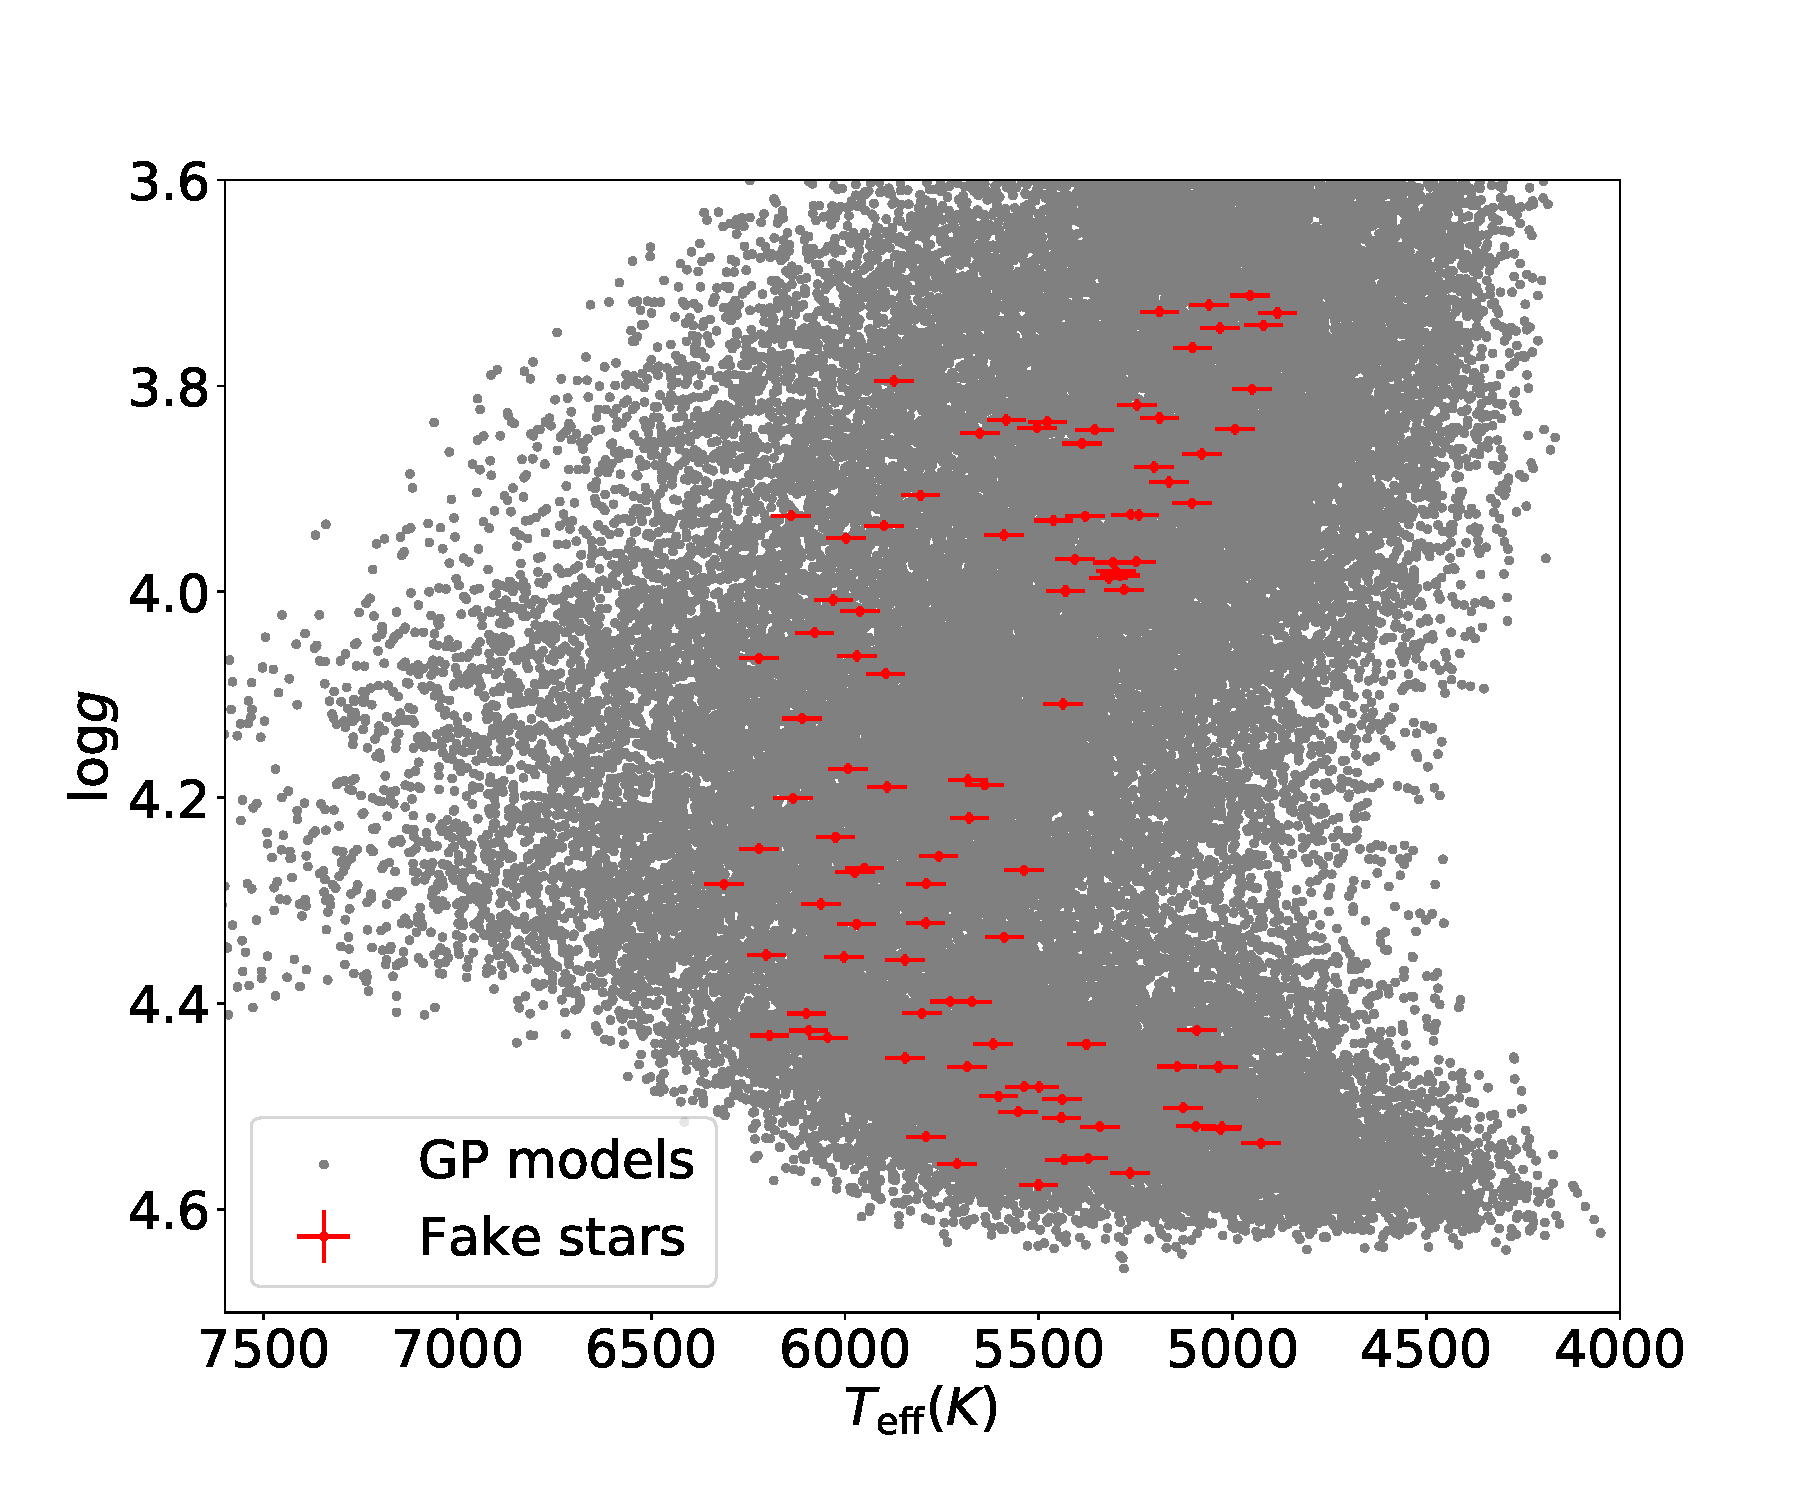
\includegraphics[width=1.0\columnwidth]{fake-stars-on-hrd.pdf}
    \caption{Fake stars. } 
  \label{fig:fit_comparison}
\end{figure}

\begin{figure*}
	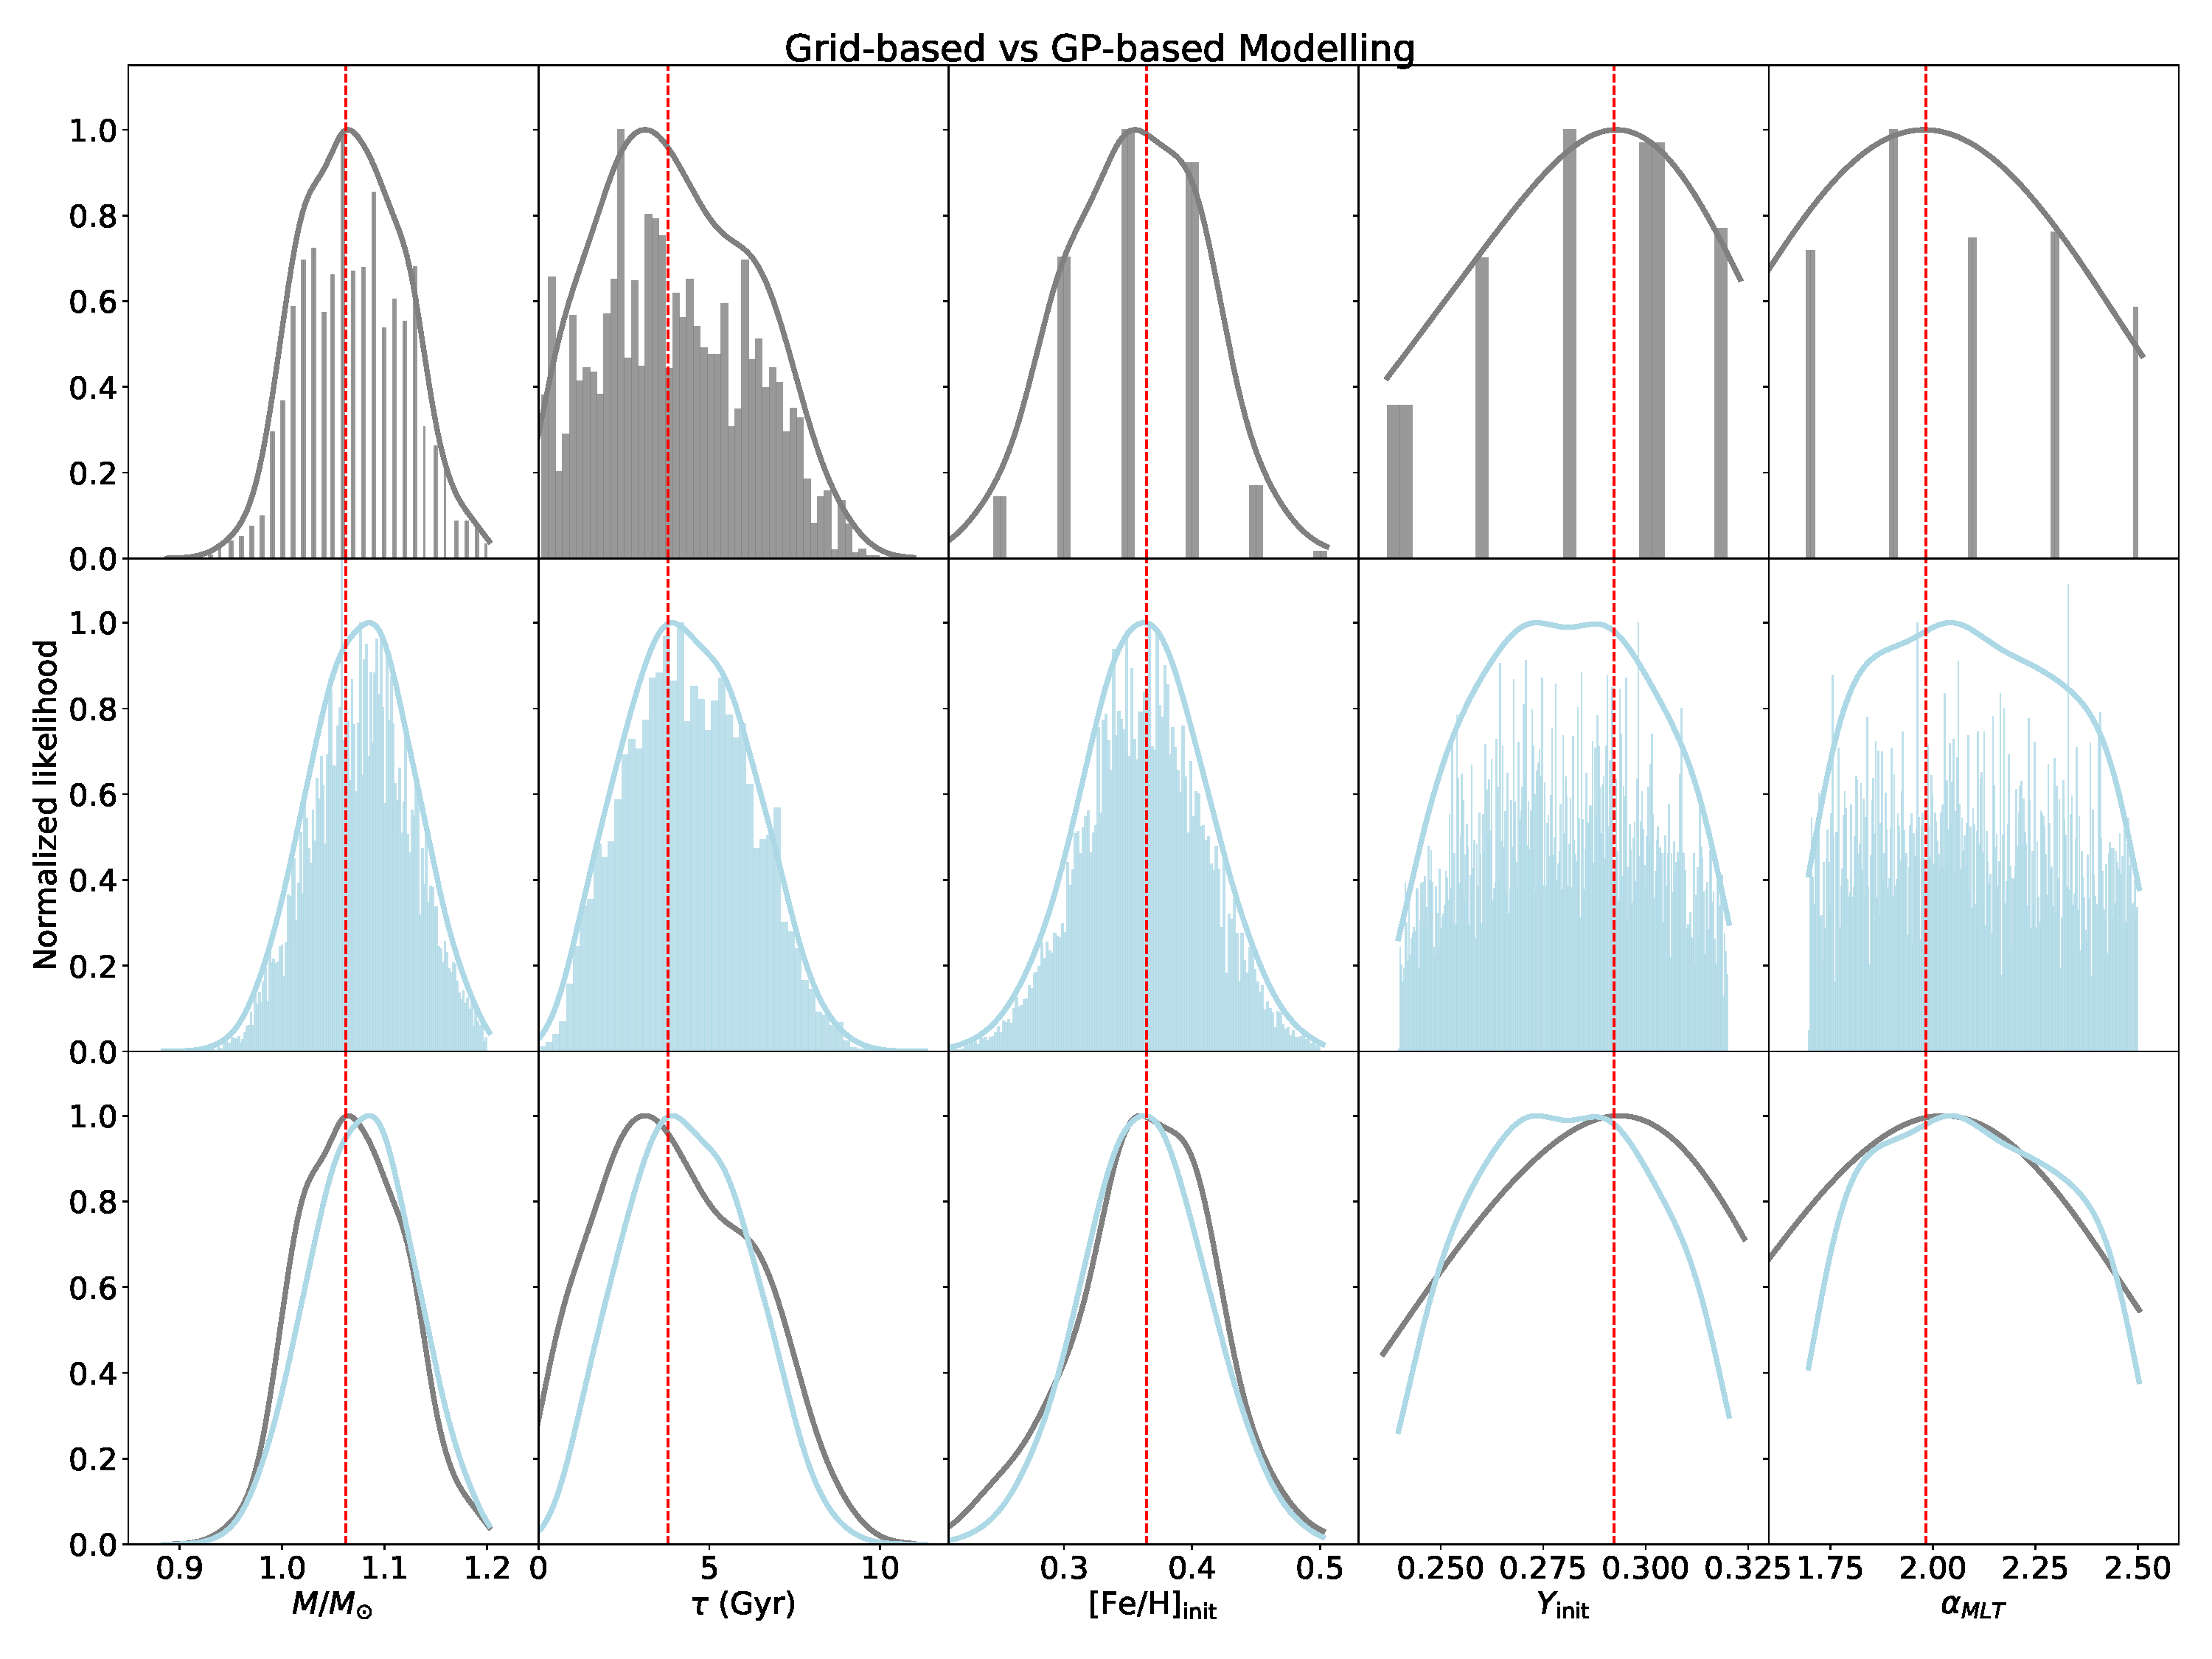
\includegraphics[width=2.0\columnwidth]{gp_fitting.pdf}
    \caption{Probability distributions of estimated fundamental parameters from grid-based and GP-based modelling. } 
  \label{fig:fit_comparison}
\end{figure*}


\begin{figure*}
	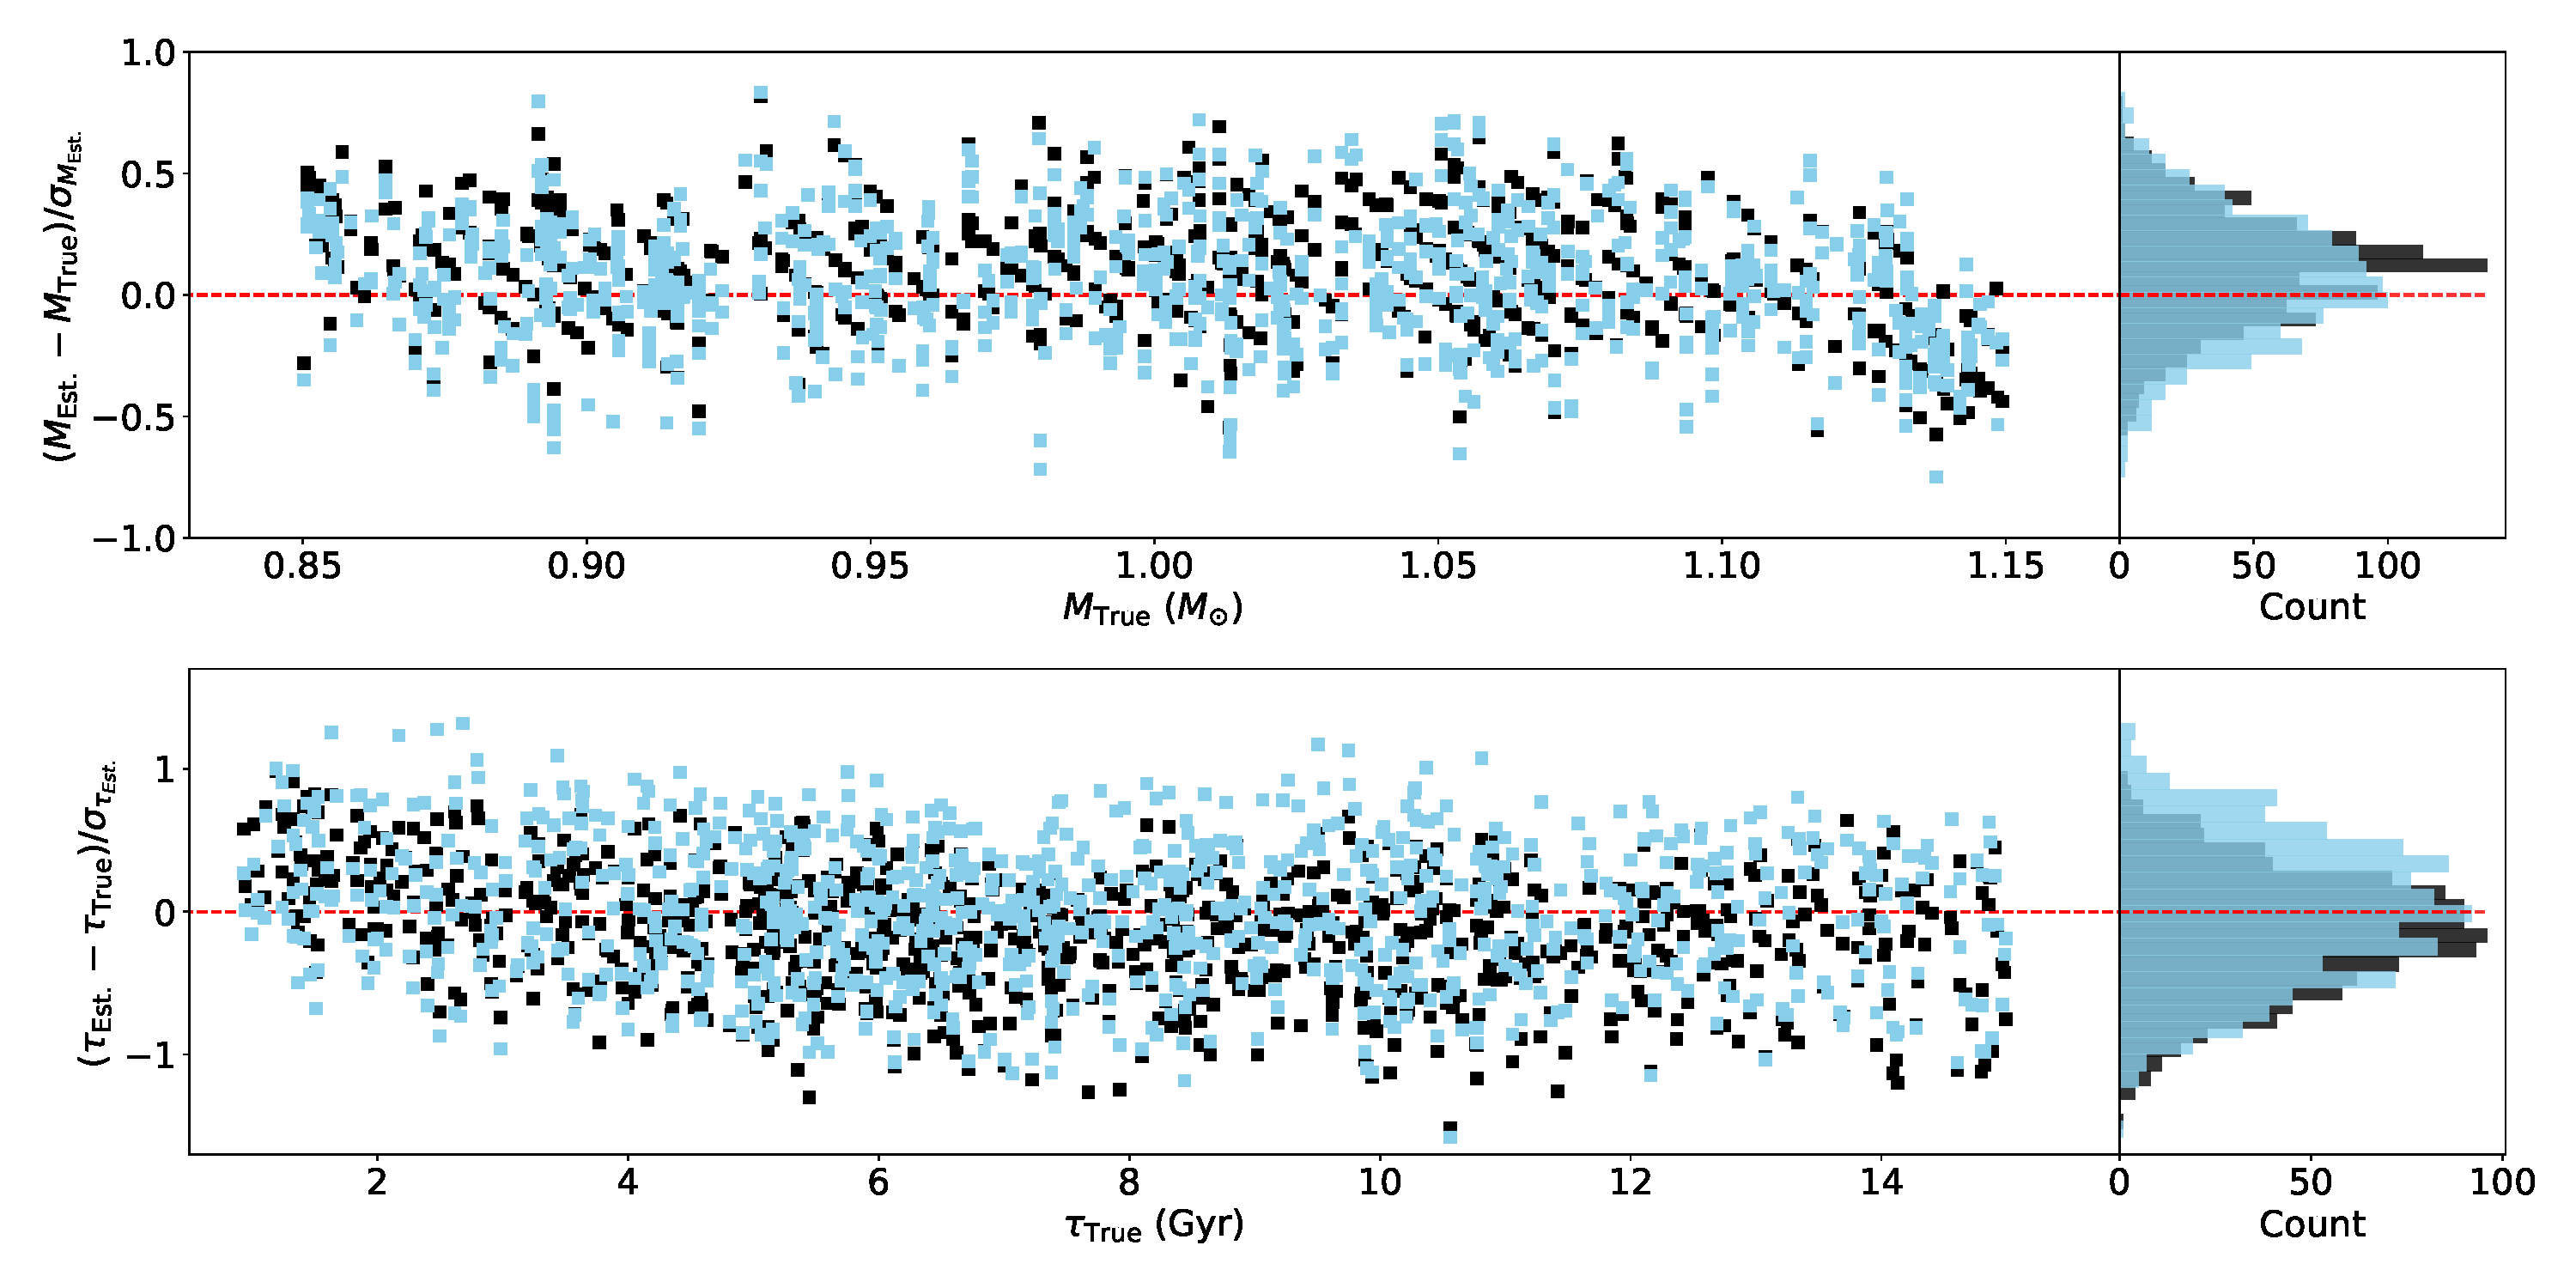
\includegraphics[width=2.0\columnwidth]{fake-stars-test.pdf}
    \caption{Results of fake stars.} 
  \label{fig:fake_test}
\end{figure*}









